\documentclass{beamer}
\usetheme{Boadilla}
\usefonttheme{serif}
\usepackage{amsmath}
\usepackage[makeroom]{cancel}
\usepackage{verbatim}
\usepackage[sort]{natbib}
\usepackage{tabularx}

\title{Gmacs}
\subtitle{A generalized size-structured stock assessment model}
\author{The Gmacs Development Team}
%\institute{Quantifish}
\date{\today}
\begin{document}

%% =========================================================================== %%

\begin{frame}
\titlepage
\end{frame}

%% =========================================================================== %%

\begin{frame}
\frametitle{Outline}
\tableofcontents
\end{frame}

%% =========================================================================== %%
%% =========================================================================== %%

\section{Notation and some definitions}

%% =========================================================================== %%
%% =========================================================================== %%

\subsection{Notation}
\begin{frame}
\frametitle{Notation}
Generally
\begin{itemize}
\item a bold capital symbol ${\bf A}$ refers to a matrix
\item a bold lowercase symbol ${\bf a}$ refers to a vector
\item an unbolded italic symbol $a$ refers to a scalar
\item $\{ a_i \}^n_{i=1}$ is an ordered $n$-tuple
\item the terms $p(\cdot)$ or $\pi(\cdot)$ represent probability
  distributions
\item $a|b$ means event $a$ conditional on event $b$ having occurred
\item the symbol $\forall$ means for all values, usually referring to all of the
  values within an ordered tuple.
\item we use \textcolor{red}{red} to indicate an estimable parameter
\item we use \textcolor{blue}{blue} to represent covariates and fixed parameters
\item we use \textcolor{green}{green} to represent data
\end{itemize}
\end{frame}

%% =========================================================================== %%

\subsection{Indices}
\begin{frame}
\frametitle{Indices}
\begin{table}
  \centering
  \begin{tabular}{cl}
  \hline
  Symbol  & Description \\
  \hline
      $g$ & group \\
      $h$ & sex \\
      $i$ & year \\
      $j$ & time step (years) \\
      $k$ & gear or fleet \\
      $\ell$ & index for size class \\
      $m$ & index for maturity state \\
      $o$ & index for shell condition \\
  \hline
  \end{tabular}
\end{table}
Notice no area index.
\end{frame}

%% =========================================================================== %%

\subsection{Leading model parameters}
\begin{frame}
\frametitle{Leading model parameters}
\begin{table}
  \centering
  \begin{tabular}{ccl}
  \hline
  Symbol & Support & Description \\
  \hline
      \textcolor{red}{$M_0$} & $0 < \textcolor{red}{M_0} < \infty$ & Initial instantaneous natural mortality rate\\
      \textcolor{red}{$R_0$} & $0 < \textcolor{red}{R_0} < \infty$ & Unfished average recruitment\\
      \textcolor{red}{$\ddot{R}$} & $0 < \textcolor{red}{\ddot{R}} < \infty$ & Initial recruitment\\
      \textcolor{red}{$\bar{R}$} & $0 < \textcolor{red}{\bar{R}} < \infty$ & Average recruitment\\
      \textcolor{red}{$\alpha_r$} & $\textcolor{red}{\alpha_r} > 0$ & Mode of size-at-recruitment\\
      \textcolor{red}{$\beta_r $} & $\textcolor{red}{\beta_r} > 0$ & Shape parameter for size-at-recruitment\\
      \textcolor{red}{$\kappa$} & $\textcolor{red}{\kappa} > 1$ & Recruitment compensation ratio\\
      %\textcolor{red}{$h$} & $\textcolor{red}{h} > 1$ & Stock recruit steepness\\
      \textcolor{red}{$\rho$} & $\textcolor{red}{\rho} > 1$ & Recruitment autocorrelation\\
  \hline
  \end{tabular}
\end{table}
We group the leading model parameters into the vector
\begin{equation*}
  \textcolor{red}{\boldsymbol\theta} = \{ \textcolor{red}{M_0},
  \textcolor{red}{R_0}, \textcolor{red}{\ddot{R}}, \textcolor{red}{\bar{R}},
  \textcolor{red}{\alpha_r}, \textcolor{red}{\beta_r}, \textcolor{red}{\kappa} \}.
\end{equation*}
\end{frame}

%% =========================================================================== %%

\subsection{Cubic splines}
\begin{frame}
\frametitle{Cubic splines}
A spline is a numeric function that is piecewise-defined by polynomial
functions, and which possesses a sufficiently high degree of smoothness at the
places where the polynomial pieces connect (which are known as knots). A cubic
spline is constructed of piecewise third-order polynomials. The second
derivative of each polynomial is commonly set to zero at the endpoints, since
this provides a boundary condition that completes the system of $m-2$
equations. This produces a so-called ``natural'' cubic spline and leads to a
simple tridiagonal system which can be solved easily to give the coefficients of
the polynomials. However, this choice is not the only one possible, and other
boundary conditions can be used instead.
\end{frame}

%% =========================================================================== %%
%% =========================================================================== %%

\section{Growth}

%% =========================================================================== %%
%% =========================================================================== %%

\begin{frame}
\frametitle{Growth parameters}
\begin{table}
  \centering
  \begin{tabular}{ccl}
  \hline
  Symbol & Support & Description \\
  \hline
      \textcolor{red}{$\alpha_h$} & $\textcolor{red}{\alpha_h} > 0$ & Mode of size-at-recruitment\\
      \textcolor{red}{$\beta_h$} & $\textcolor{red}{\beta_h} > 0$ & Shape parameter for size-at-recruitment\\
      \textcolor{red}{$\varphi_h$} & $\textcolor{red}{\varphi_h} > 0$ & Instantaneous natural mortality rate\\
      \textcolor{red}{$\mu_h$} & $\textcolor{red}{\mu_h} > 0$ & Length at 50\% molting probability\\
      \textcolor{red}{$c_h$} & $\textcolor{red}{c_h} > 0$ & Coefficient of variation of molting probability\\
  \hline
  \end{tabular}
\end{table}
We group the growth parameters into the vector
\begin{equation*}
  \textcolor{red}{\boldsymbol\psi} = \{ \textcolor{red}{\alpha_h}, 
  \textcolor{red}{\beta_h}, \textcolor{red}{\varphi_h}, \textcolor{red}{\mu_h},
  \textcolor{red}{c_h} \}.
\end{equation*}
\end{frame}

%% =========================================================================== %%

\begin{frame}
\frametitle{Growth matrix}
The average molt increment from size class $\ell$ to $\ell'$ is assumed to be
sex-specific and is defined by the linear function
\begin{equation*}
  a_{h,\ell} = \frac{\textcolor{red}{\alpha_h} + \textcolor{red}{\beta_h}
    \ell}{\textcolor{red}{\varphi_h}}.
\end{equation*}
The probability of transitioning from size class $\ell$ to $\ell'$ assumes that
variation in molt increments follows a gamma distribution
\begin{equation*}
  p (\ell'|\ell)_h = \boldsymbol{G}_h = \int^{\ell + \Delta \ell}_\ell \frac{\ell^{a_{h,\ell-1}} \exp
    \left(\frac{\ell}{\textcolor{red}{\varphi_h}} \right)}{\Gamma (a_{h,\ell}) \ell^{a_{h,\ell}}}
  \quad \text{where} \quad \Delta \ell = \ell' - \ell.
\end{equation*}
Specifically
\begin{equation*}
  \boldsymbol{G} = G_{\ell,\ell'} = \left( \begin{array}{cccc}
      G_{1,1} & G_{1,2} & \hdots & G_{1,n} \\
      G_{2,1} & G_{2,2} & \hdots & G_{2,n} \\
      \vdots & \vdots & \ddots & \vdots \\
      G_{n,1} & G_{n,2} & \hdots & G_{n,n} \end{array} \right)
  \quad \text{where} \quad \sum_{\ell'} G_{\ell,\ell'} = 1 \quad \forall \ell.
\end{equation*}
\end{frame}

%% =========================================================================== %%

\begin{frame}
\frametitle{Growth increments ($a_{h,\ell}$)}
\begin{figure}[!htbp]
  \centering
  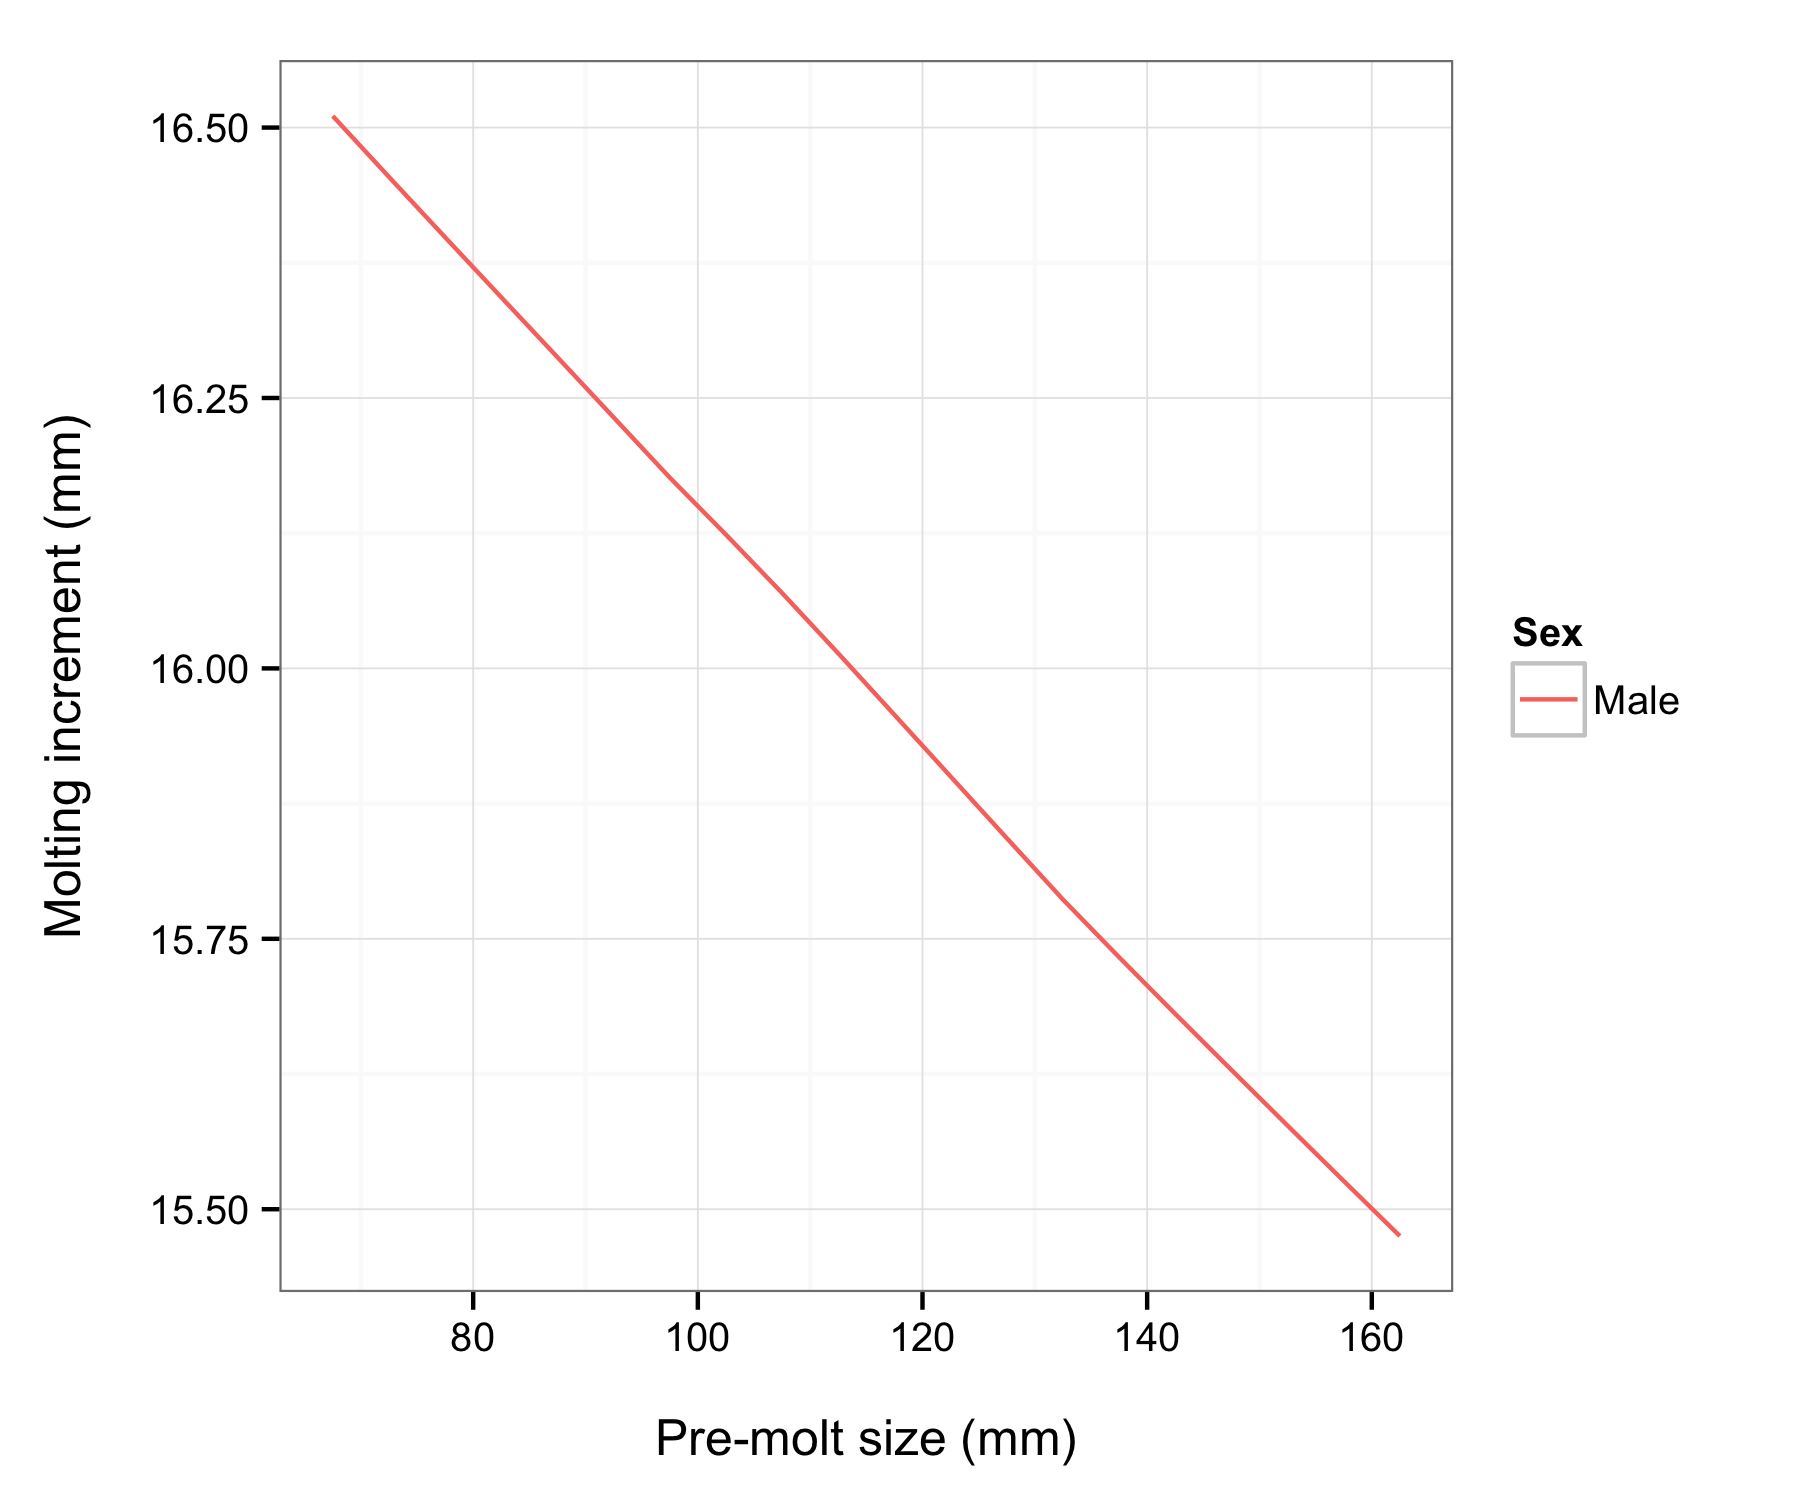
\includegraphics[width=0.75\linewidth]{../../examples/bbrkc/OneSex/figure/gi.png}
\end{figure}
\end{frame}

%% =========================================================================== %%

\begin{frame}
\frametitle{Growth transitions ($\boldsymbol{G}_h$)}
\begin{figure}[!htbp]
  \centering
  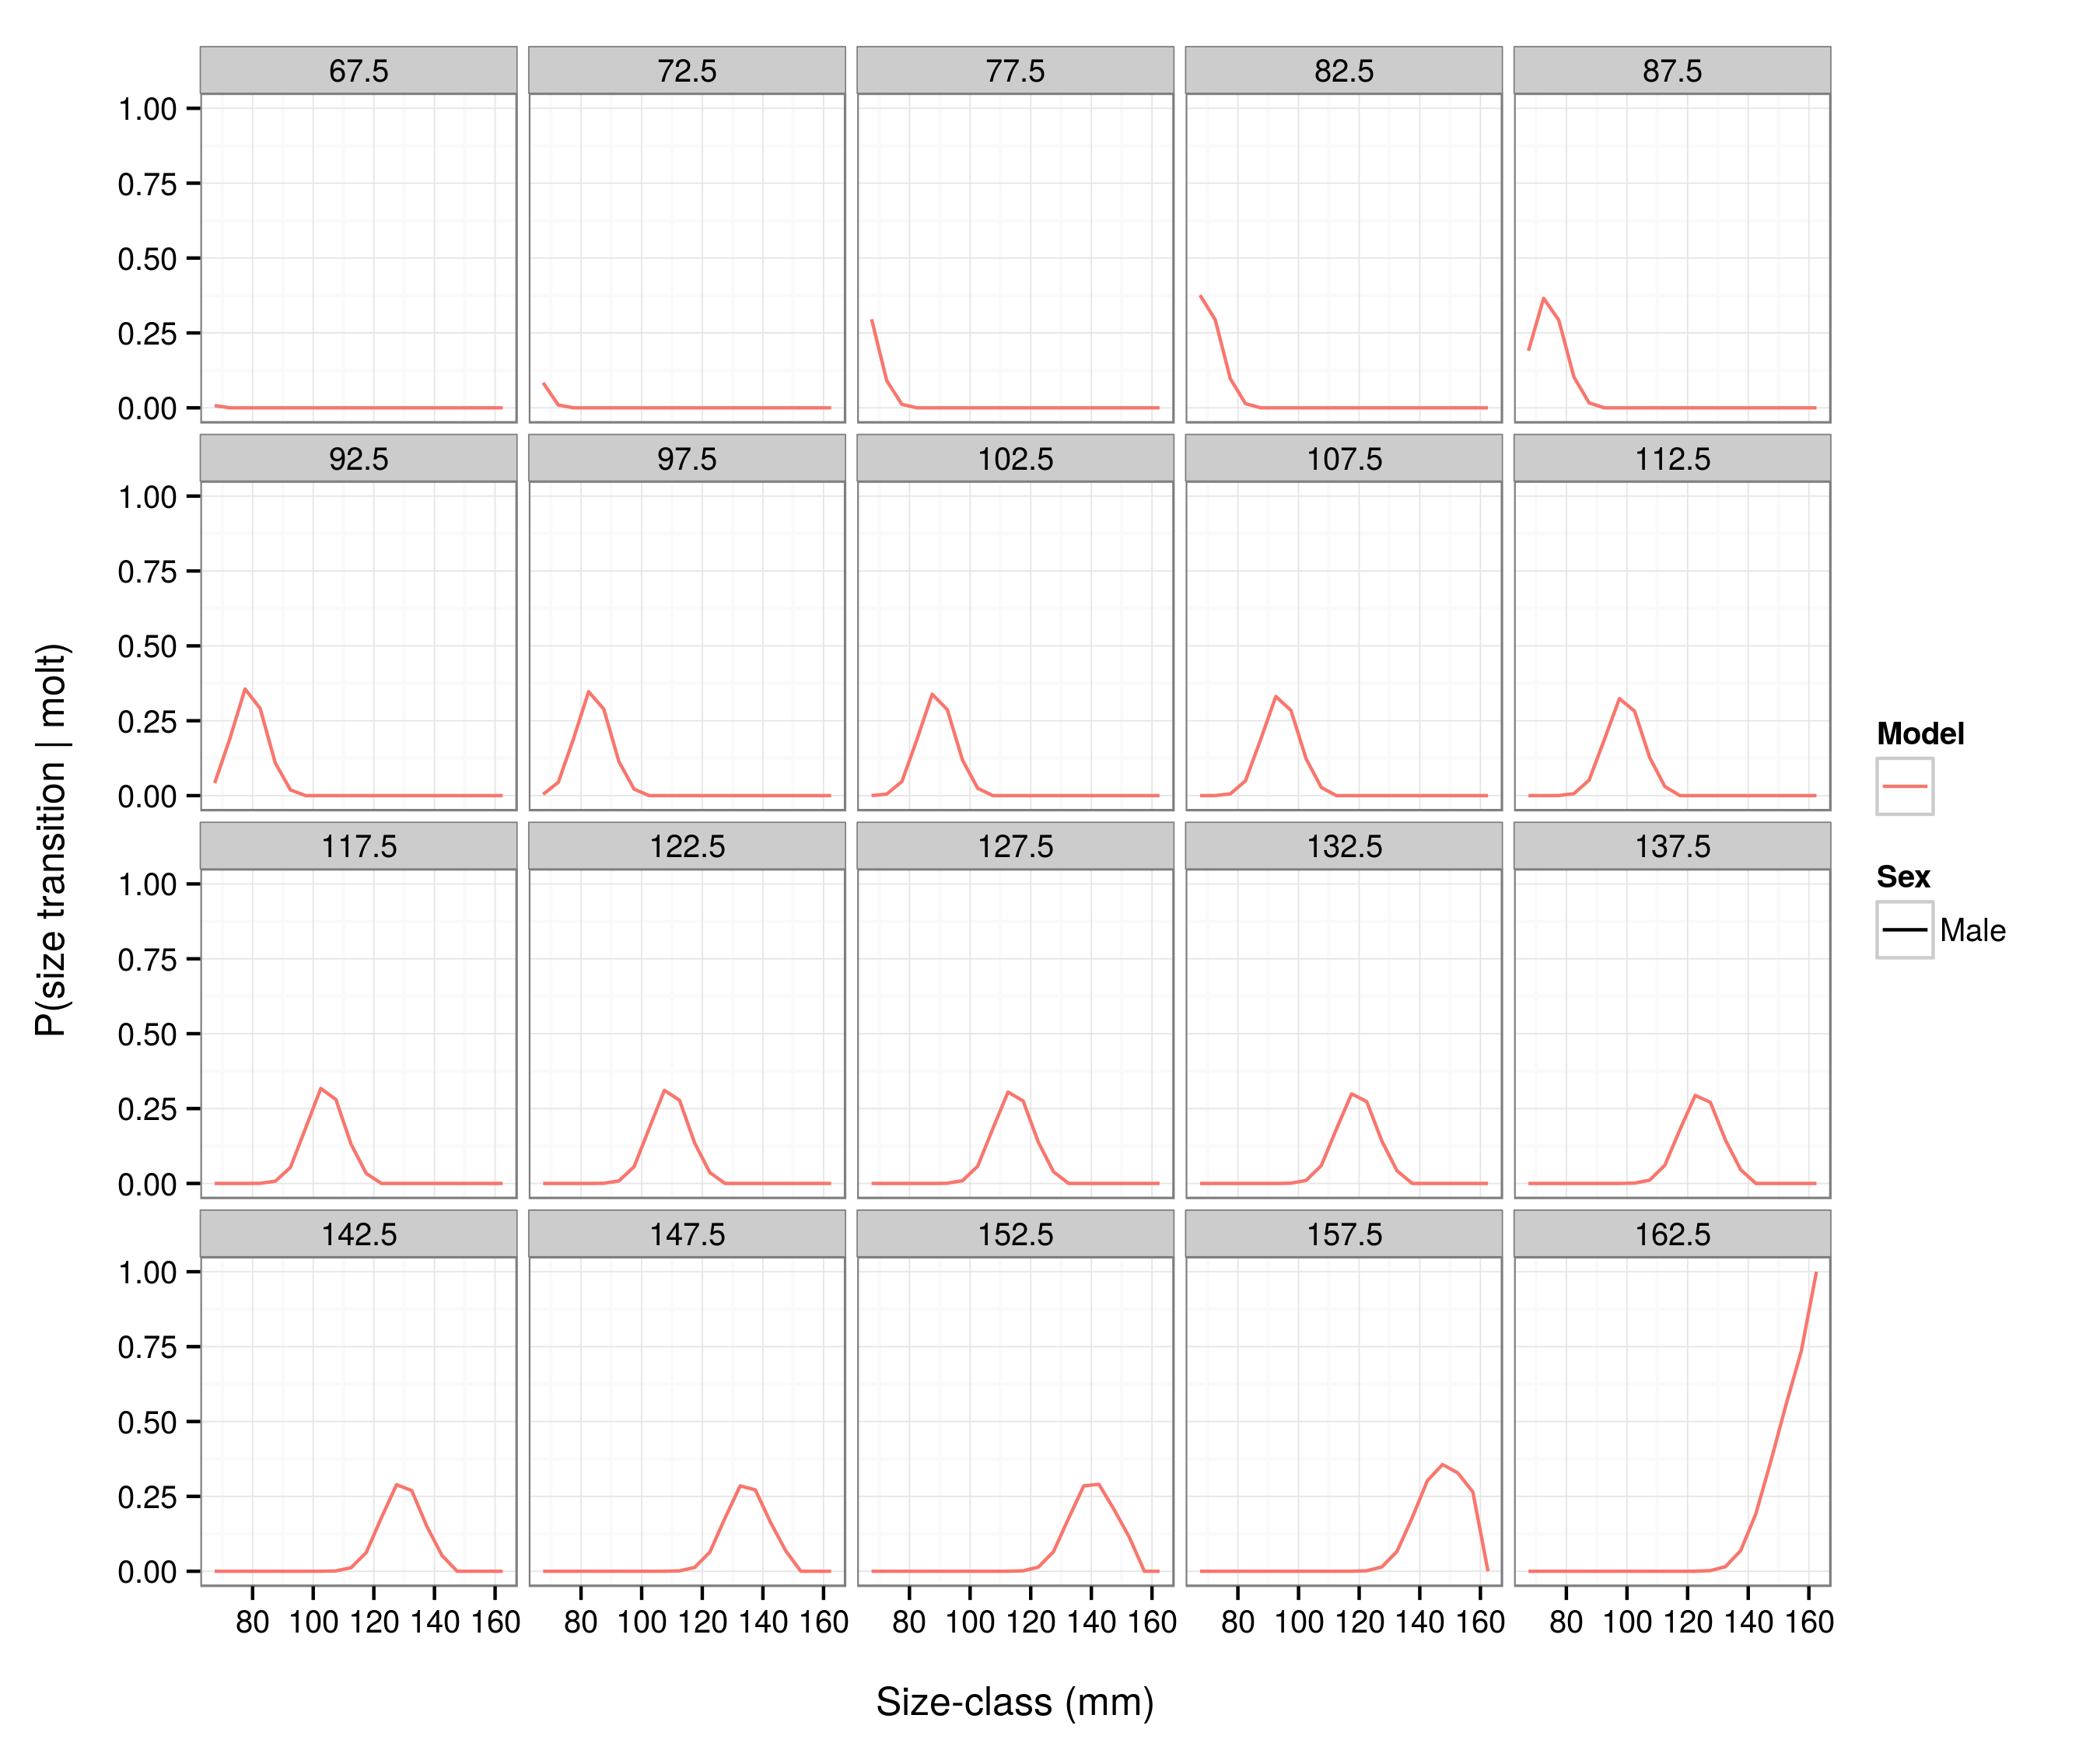
\includegraphics[width=0.75\linewidth]{../../examples/bbrkc/OneSex/figure/growth_transition.png}
\end{figure}
\end{frame}

%% =========================================================================== %%

\subsection{Molting}
\begin{frame}
\frametitle{Molting probability ($\boldsymbol{P}_h$)}
The standard deviation of molting probability ($\textcolor{red}{\sigma_h}$) is
calculated from the length at 50\% molting probability
($\textcolor{red}{\mu_h}$) coefficient of variation of molting probability
($\textcolor{red}{c_h}$) as
\begin{equation*}
  \sigma_h = \textcolor{red}{\mu_h} \textcolor{red}{c_h}.
\end{equation*}
The molting probability ($\boldsymbol{P}_h$) is calculated as
\begin{equation*}
  \boldsymbol{P}_h = 1 + (-1 - \exp(\textcolor{red}{\mu_h} - \ell) / \sigma_h)^{-1}.
\end{equation*}
The molting probability ($\boldsymbol{P}_h$) and the growth probability
($\boldsymbol{G}_h$) are combined to yield the size transition matrix
($\boldsymbol{P}_h \boldsymbol{G}_h$).
\end{frame}

%% =========================================================================== %%

\begin{frame}
\frametitle{Molting probability ($\boldsymbol{P}_h$)}
\begin{figure}[!htbp]
  \centering
  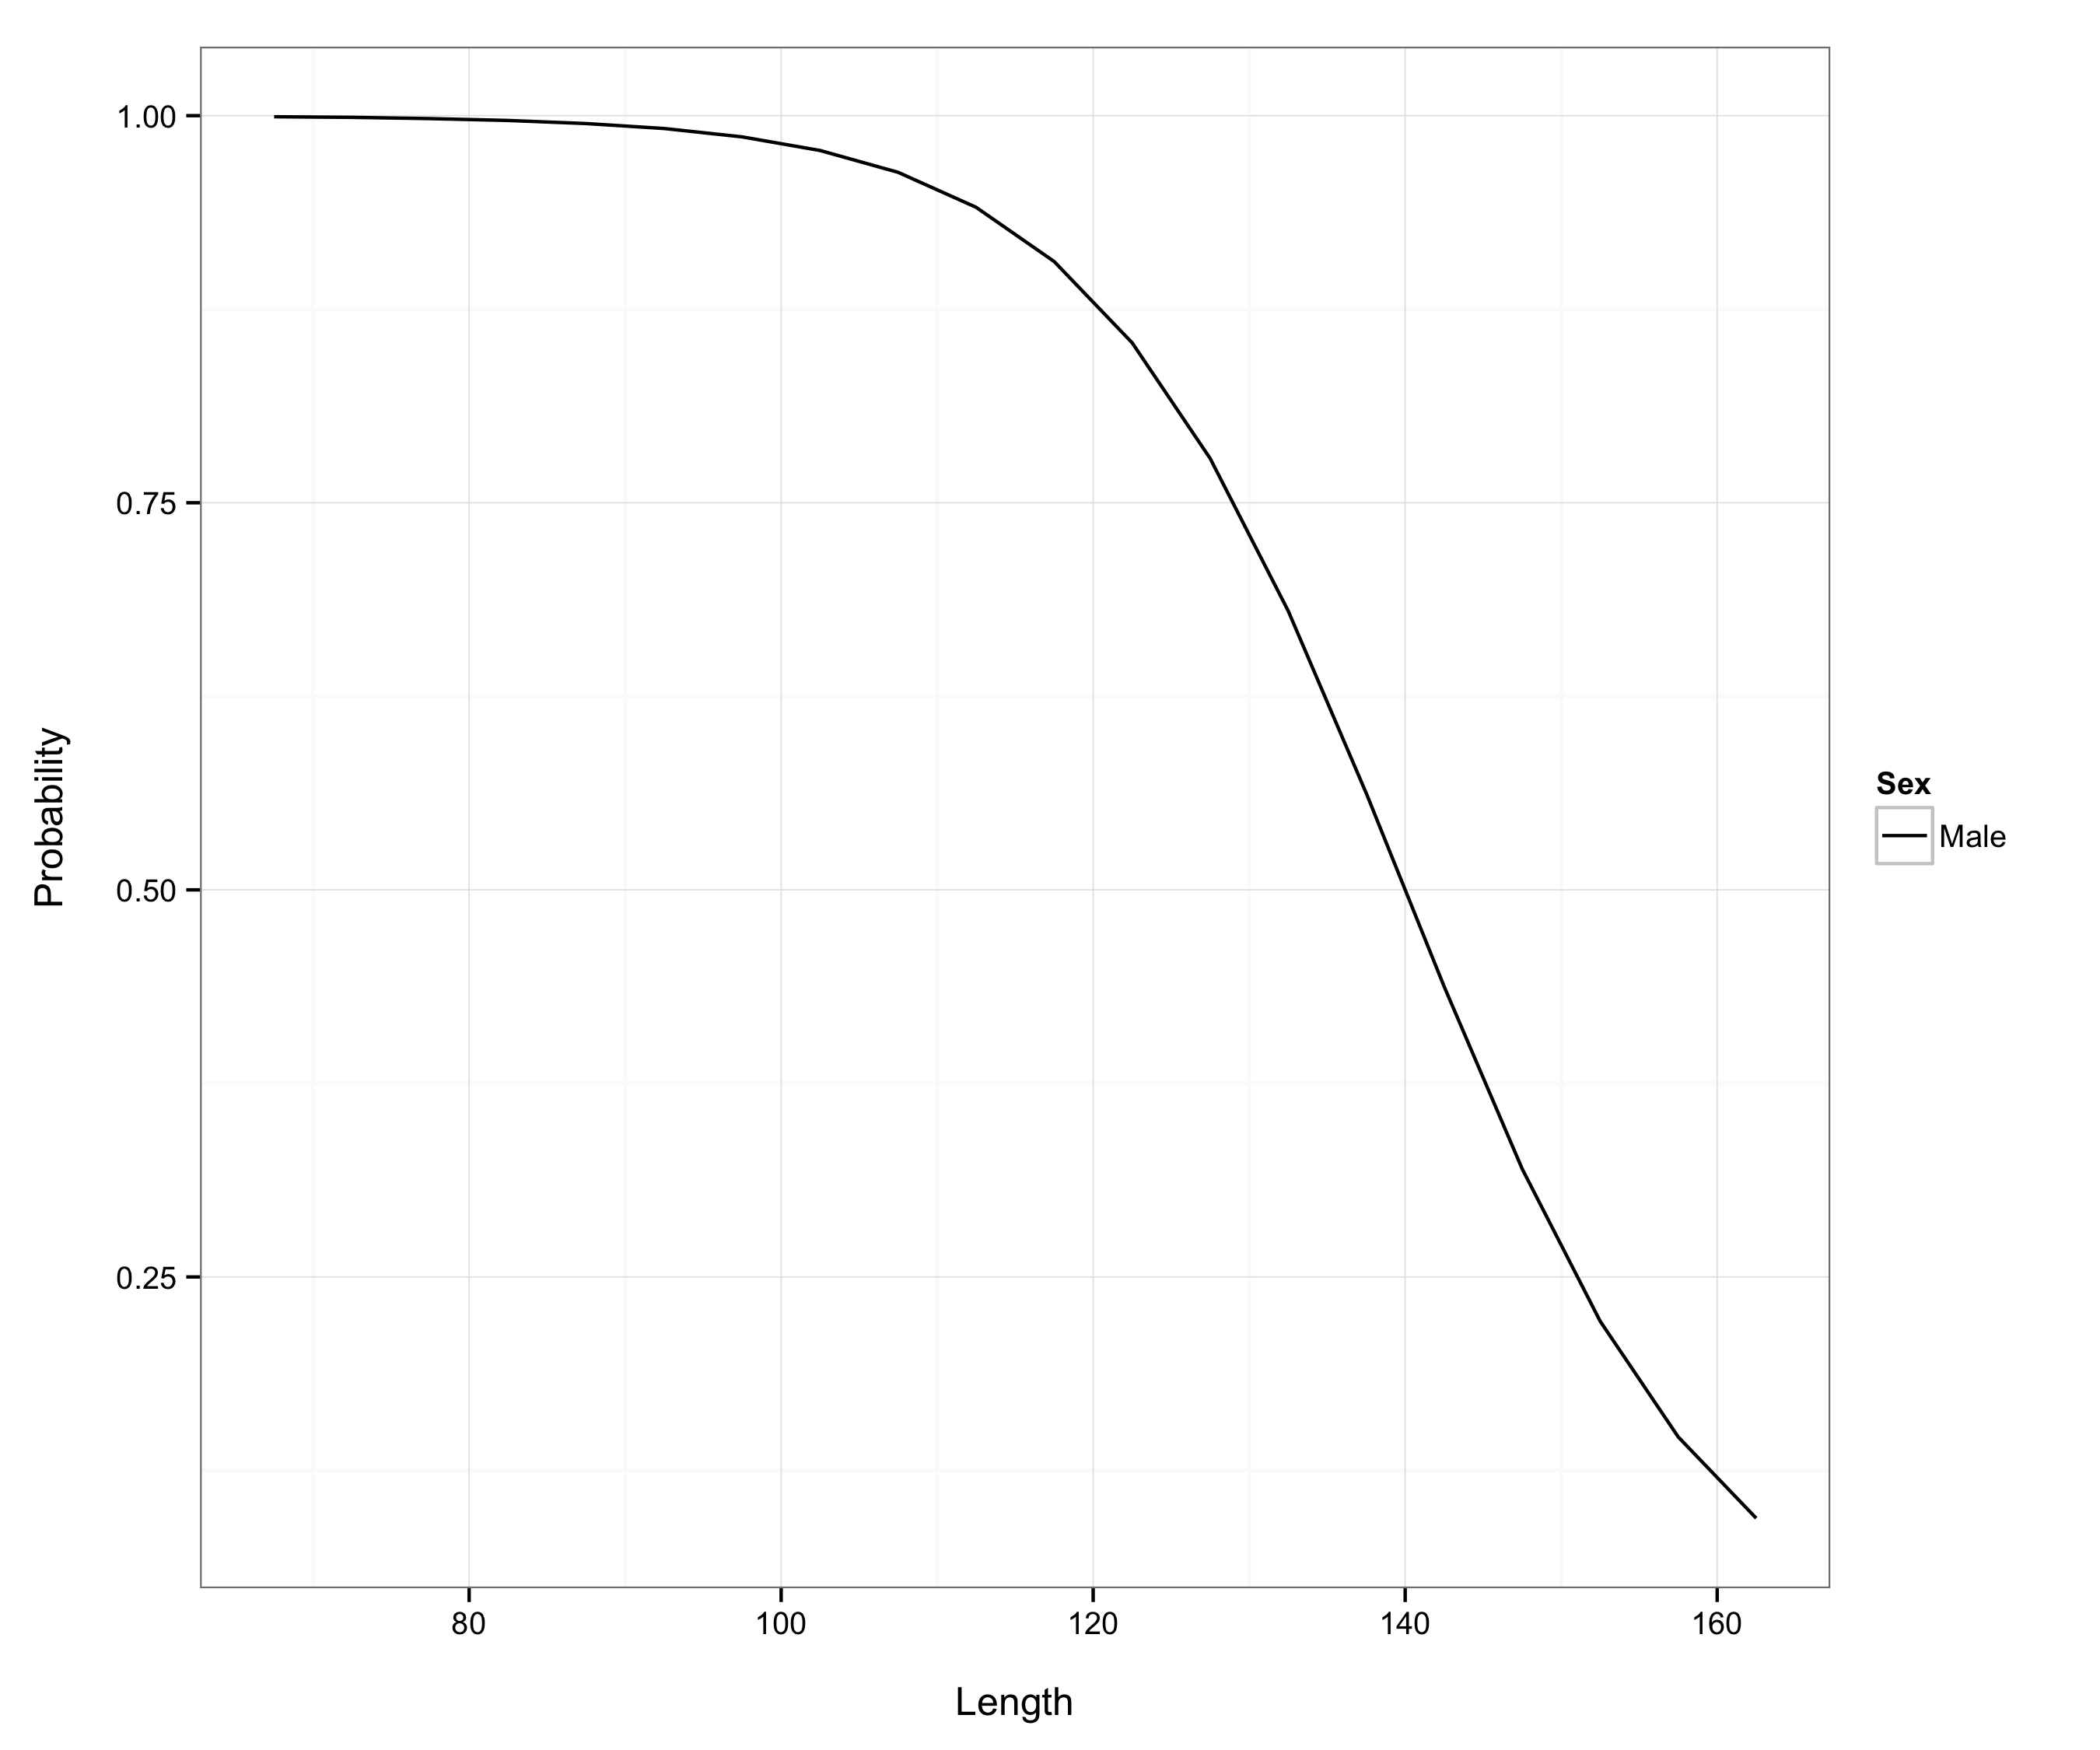
\includegraphics[width=0.75\linewidth]{../../examples/bbrkc/OneSex/figure/molt_prob.png}
\end{figure}
\end{frame}

%% =========================================================================== %%

\begin{frame}
\frametitle{Size transitions  ($\boldsymbol{P}_h \boldsymbol{G}_h$)}
\begin{figure}[!htbp]
  \centering
  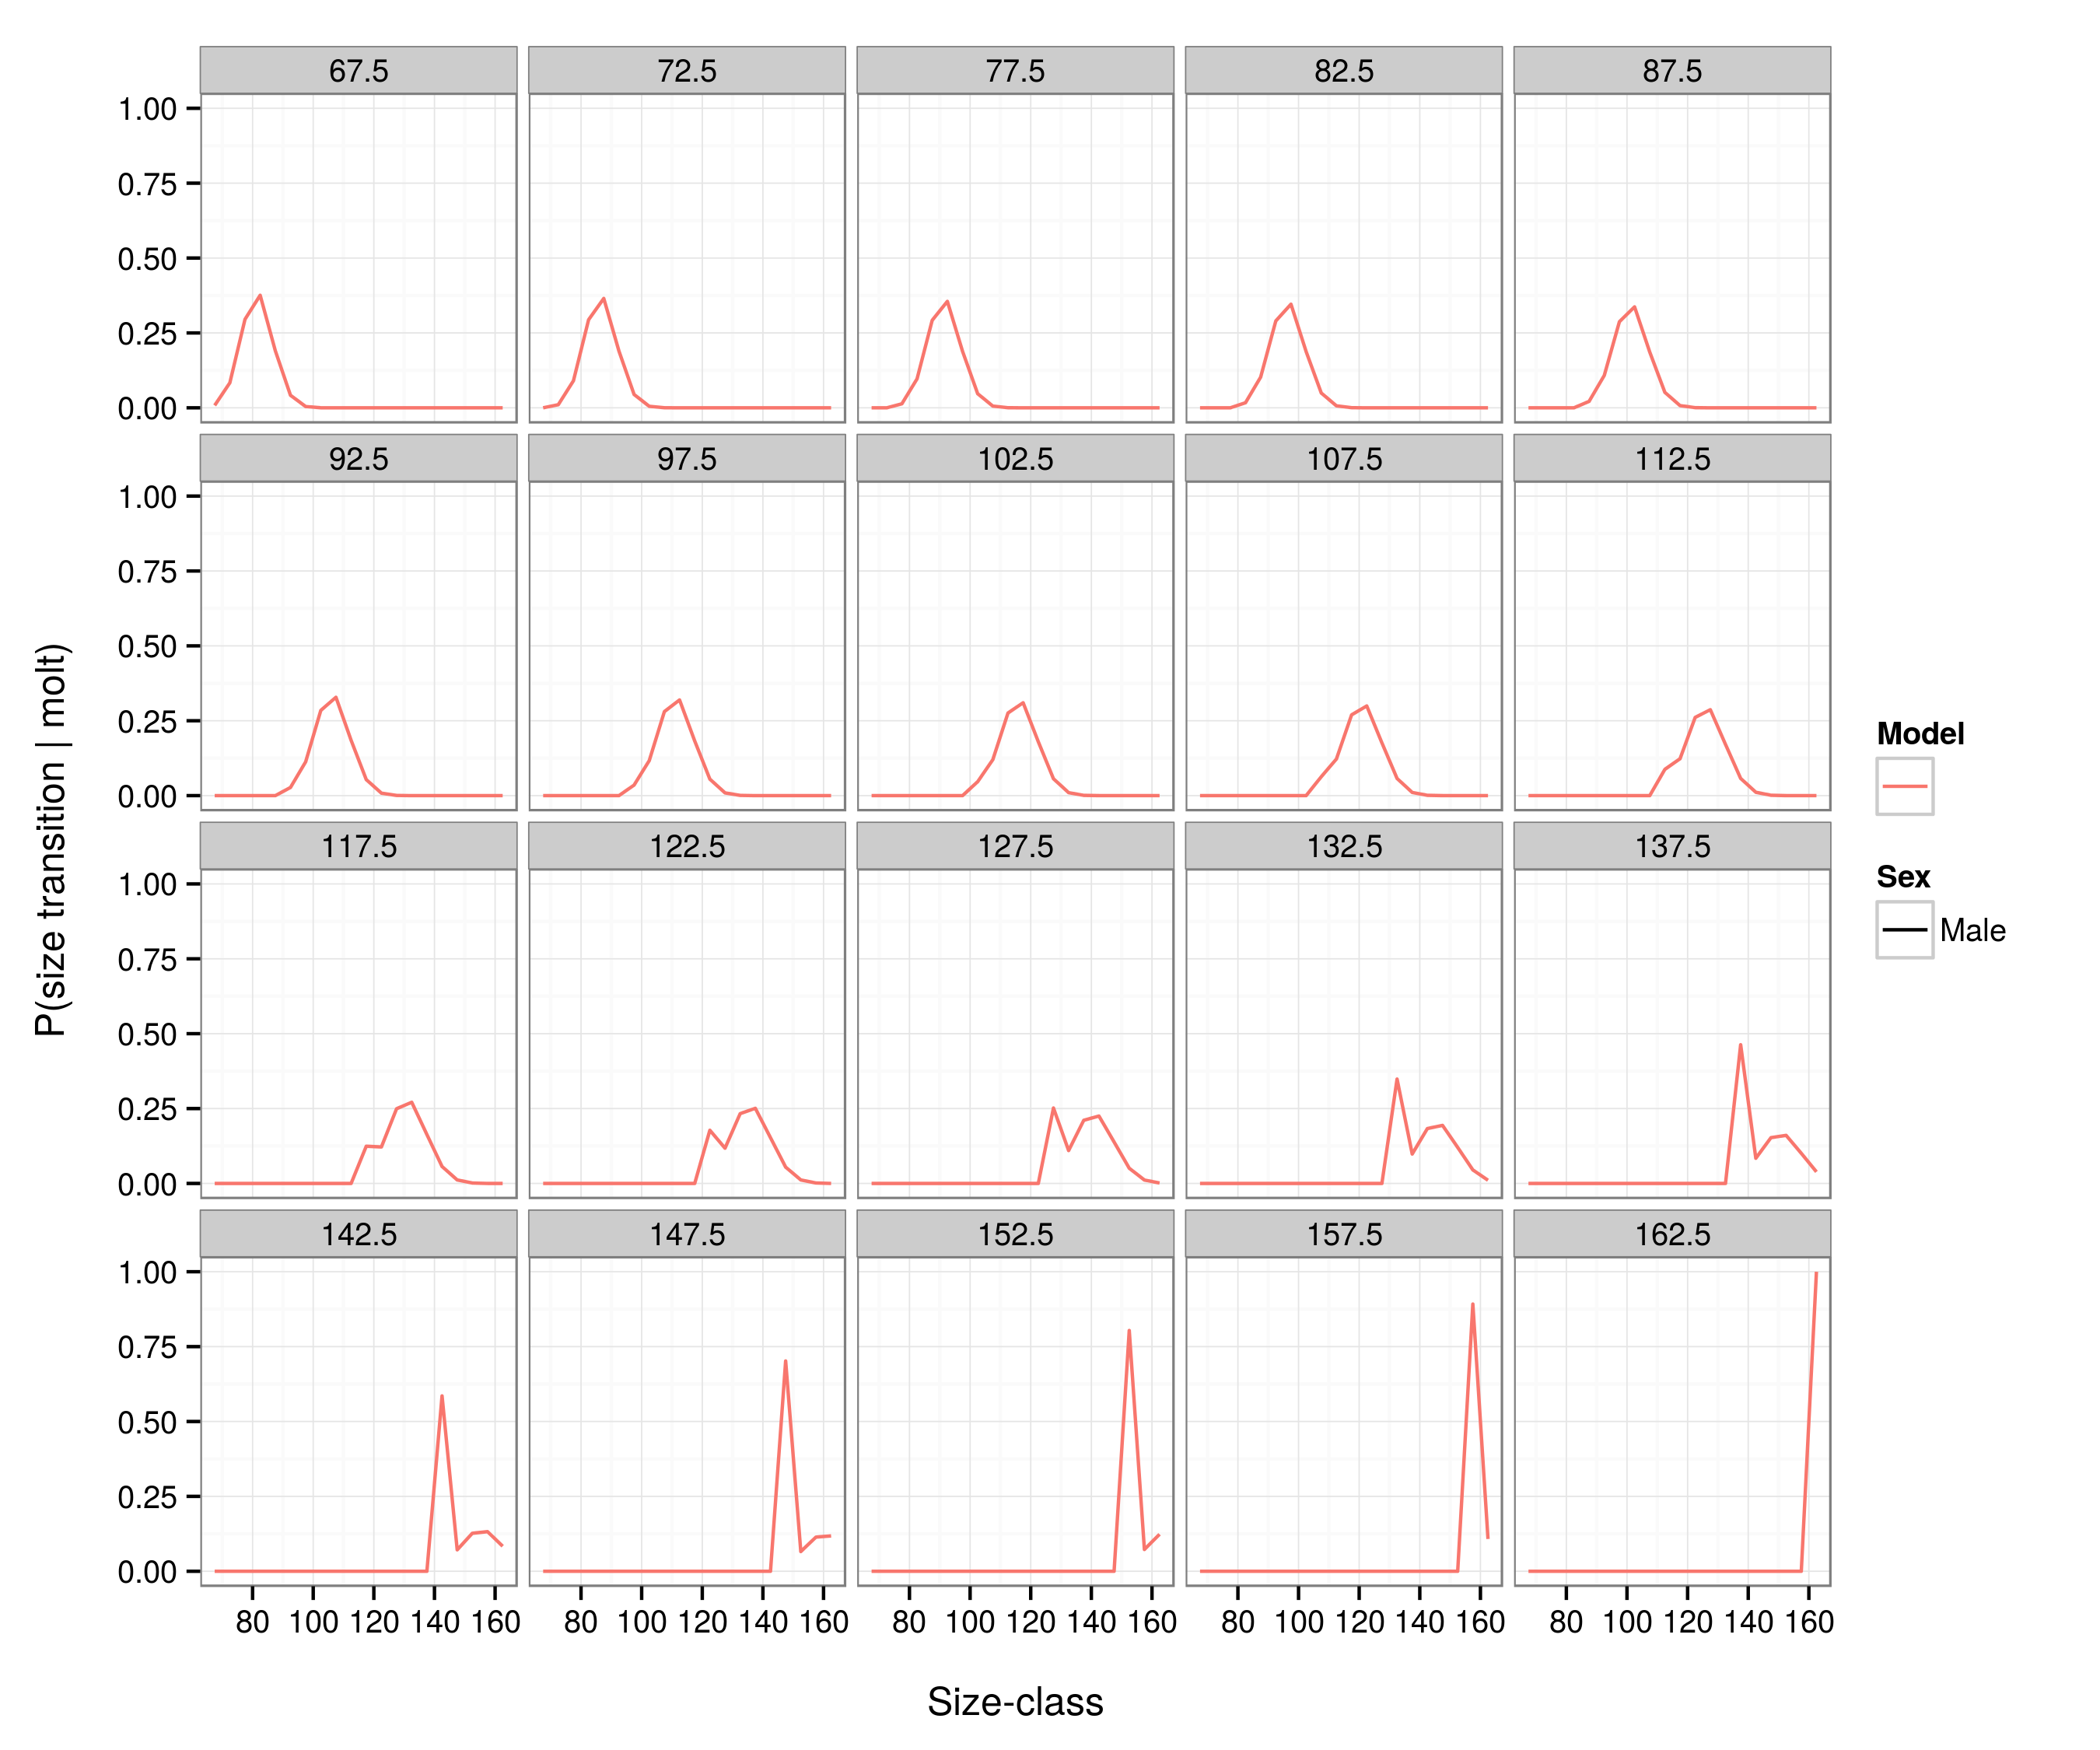
\includegraphics[width=0.75\linewidth]{../../examples/bbrkc/OneSex/figure/size_transition.png}
\end{figure}
\end{frame}

%% =========================================================================== %%
%% =========================================================================== %%

\section{Natural mortality and survival}

%% =========================================================================== %%
%% =========================================================================== %%

\subsection{Natural mortality}
\begin{frame}
\frametitle{Natural mortality variables}
\begin{table}
  \centering
  \begin{tabular}{cl}
  \hline
  Symbol  & Description \\
  \hline
      $\textcolor{red}{M_{0,h}}$ & Initial instantaneous natural mortality rate \\
      $\textcolor{blue}{\sigma_M}$ & Standard deviation of natural mortality \\
      $\delta_i$ & Natural mortality deviate \\
      $\textcolor{red}{M_{h,i}}$ & Natural mortality by sex $h$ and year $i$ \\
  \hline
  \end{tabular}
\end{table}
\end{frame}

%% =========================================================================== %%

\begin{frame}
\frametitle{Natural mortality options}
Natural mortality ($M$) is assumed to be sex-specific ($h$), size-independent
($\ell$), and may or may not be constant over time ($i$). The options currently
available in Gmacs include:
\begin{enumerate}
\item Constant natural mortality ($\textcolor{red}{M_{h,i}} = \textcolor{red}{M_{0,h}}$)
\item Random walk (deviates constrained by variance $\textcolor{blue}{\sigma^2_M}$)
\item Cubic Spline (deviates constrained by nodes and node placement)
\item Blocked changes (deviates constrained by variance in specified blocks
  $\iota \in i$)
\end{enumerate}
\end{frame}

%% =========================================================================== %%

\begin{frame}
\frametitle{Natural mortality: option 2}
If time-varying natural mortality is specified using the {\bf random walk}
option, the model constrains $M_{h,i}$ to be a random-walk process with variance
$\sigma^2_M$
\begin{equation*}
  \textcolor{red}{M_{h,i+1}} = 
  \begin{cases}
    \textcolor{red}{M_{0,h}} \quad \text{for} \quad i=1\\
    \textcolor{red}{M_{h,i}} e^{\delta_i} \quad \text{for} \quad i>1
  \end{cases},
\end{equation*}
where
\begin{equation*}
  \delta_i \sim \mathcal{N} \left( 0, \textcolor{blue}{\sigma^2_M} \right).
\end{equation*}
A time-varying natural mortality can be estimated for all years ($i$), or for
specified blocks of years ($\iota \in i$).
\end{frame}

%% =========================================================================== %%

\begin{frame}
\frametitle{Natural mortality: option 2}
Below we present an example in which time-varying natural mortality is estimated
as a {\bf random walk} process for all years ($i$)
\begin{figure}[!htbp]
  \centering
  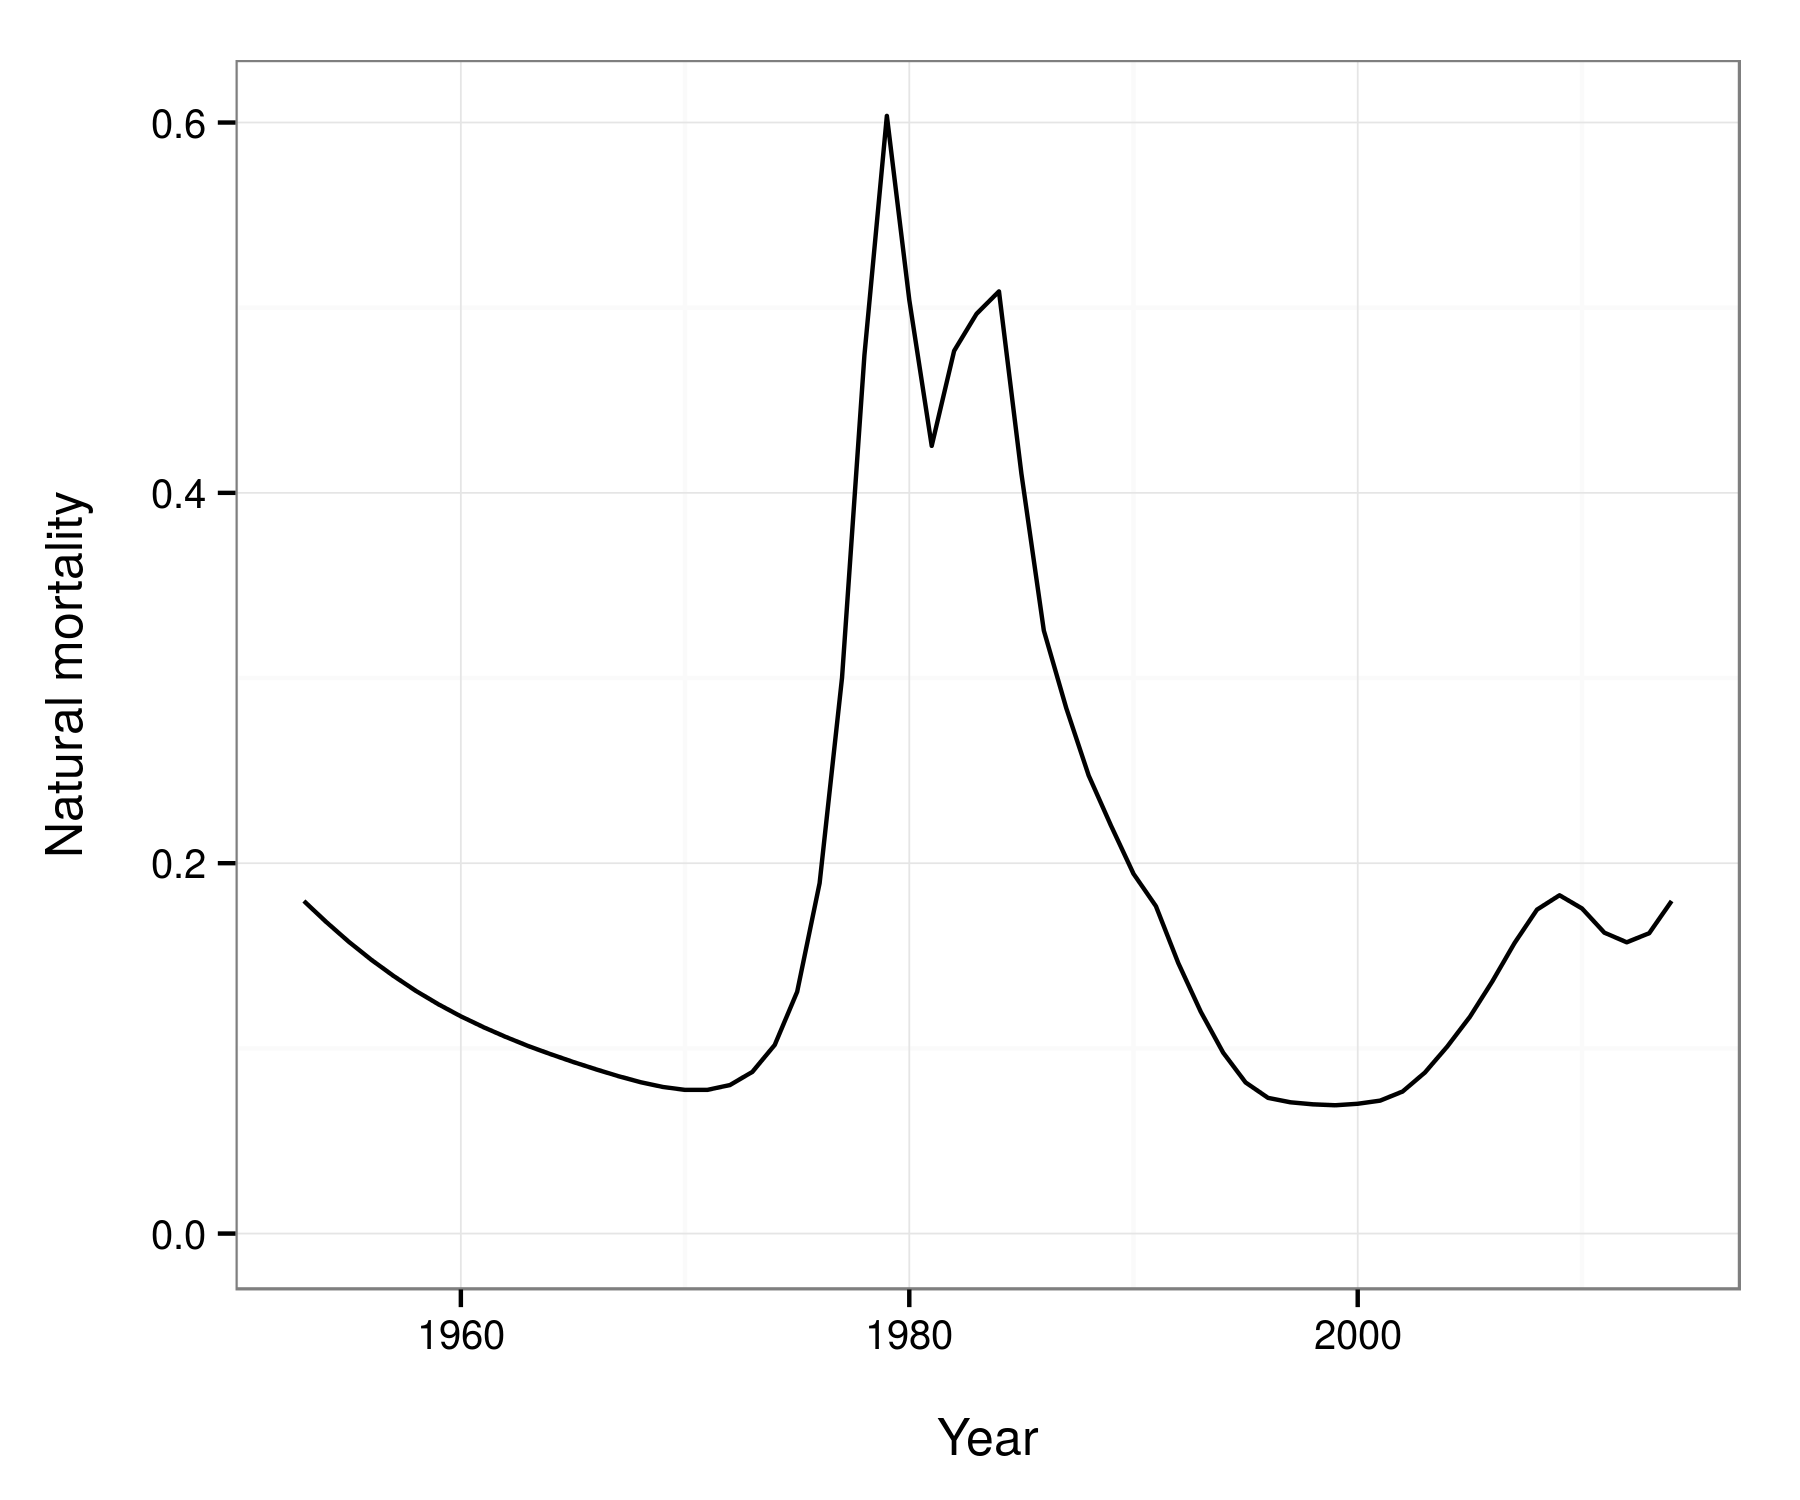
\includegraphics[width=0.65\linewidth]{figure/M_t_walk.png}
\end{figure}
\end{frame}

%% =========================================================================== %%

\begin{frame}
\frametitle{Natural mortality: option 3}
If time-varying natural mortality is specified using the {\bf cubic spline}
option, the model constrains $\textcolor{red}{M_{h,i}}$ to be a cubic spline process at
specified knots. For example, setting
\begin{figure}[!htbp]
  \centering
  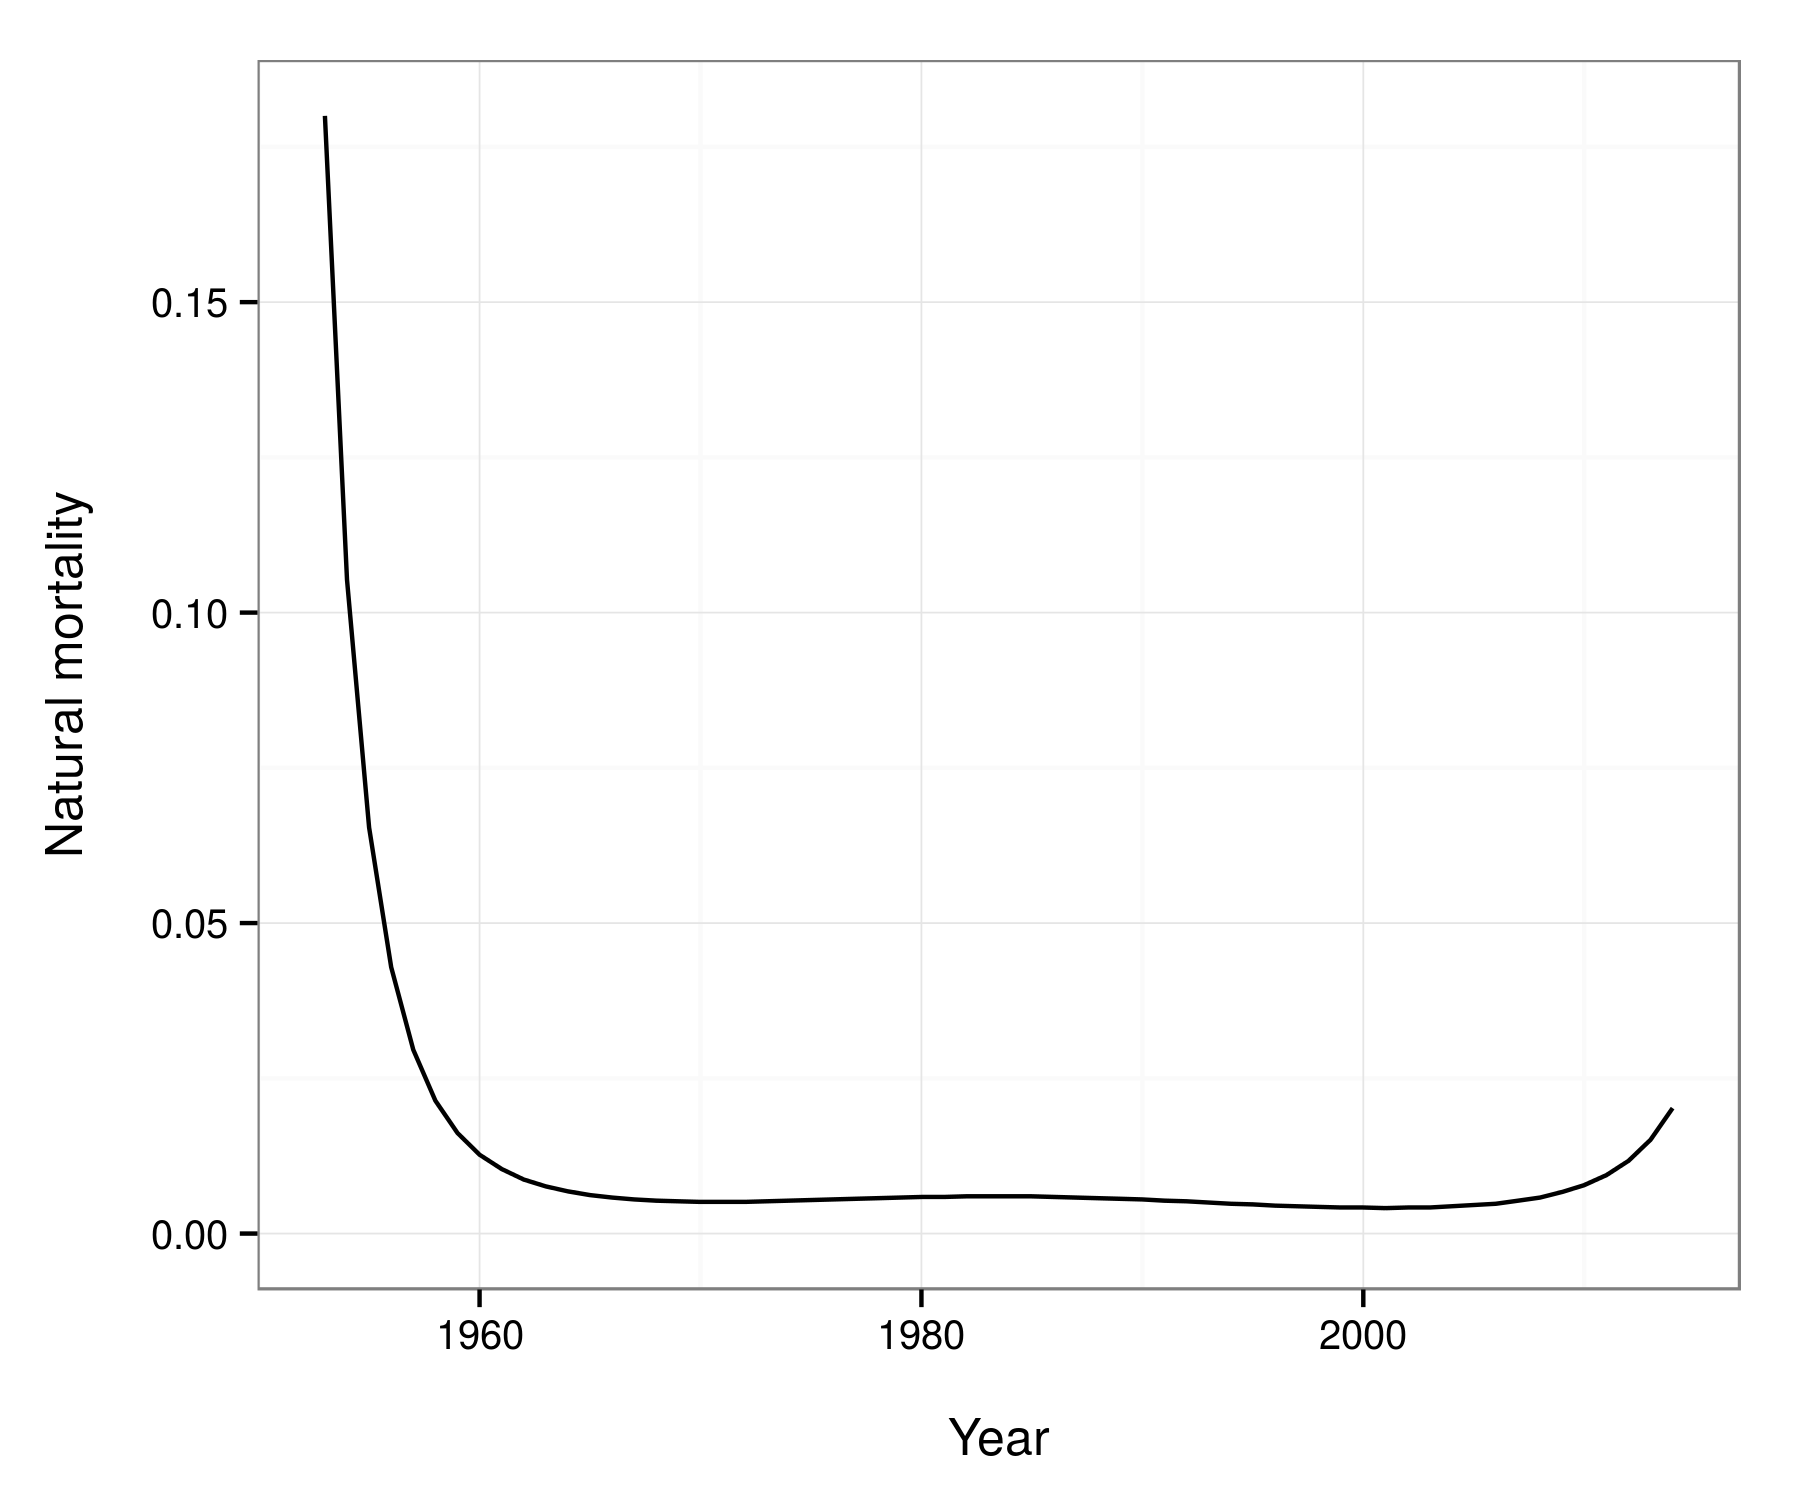
\includegraphics[width=0.65\linewidth]{figure/M_t_spline.png}
\end{figure}
\end{frame}

%% =========================================================================== %%

\begin{frame}
\frametitle{Natural mortality: option 4}
If time-varying natural mortality is specified using the {\bf blocked changes}
option, the model constrains $\textcolor{red}{M_{h,i}}$ by the variance
($\textcolor{blue}{\sigma^2_M}$). For example, setting
$\textcolor{blue}{\sigma^2_M} = 0.04$ and four specific years (1976, 1980, 1985,
1994) we get
\begin{figure}[!htbp]
  \centering
  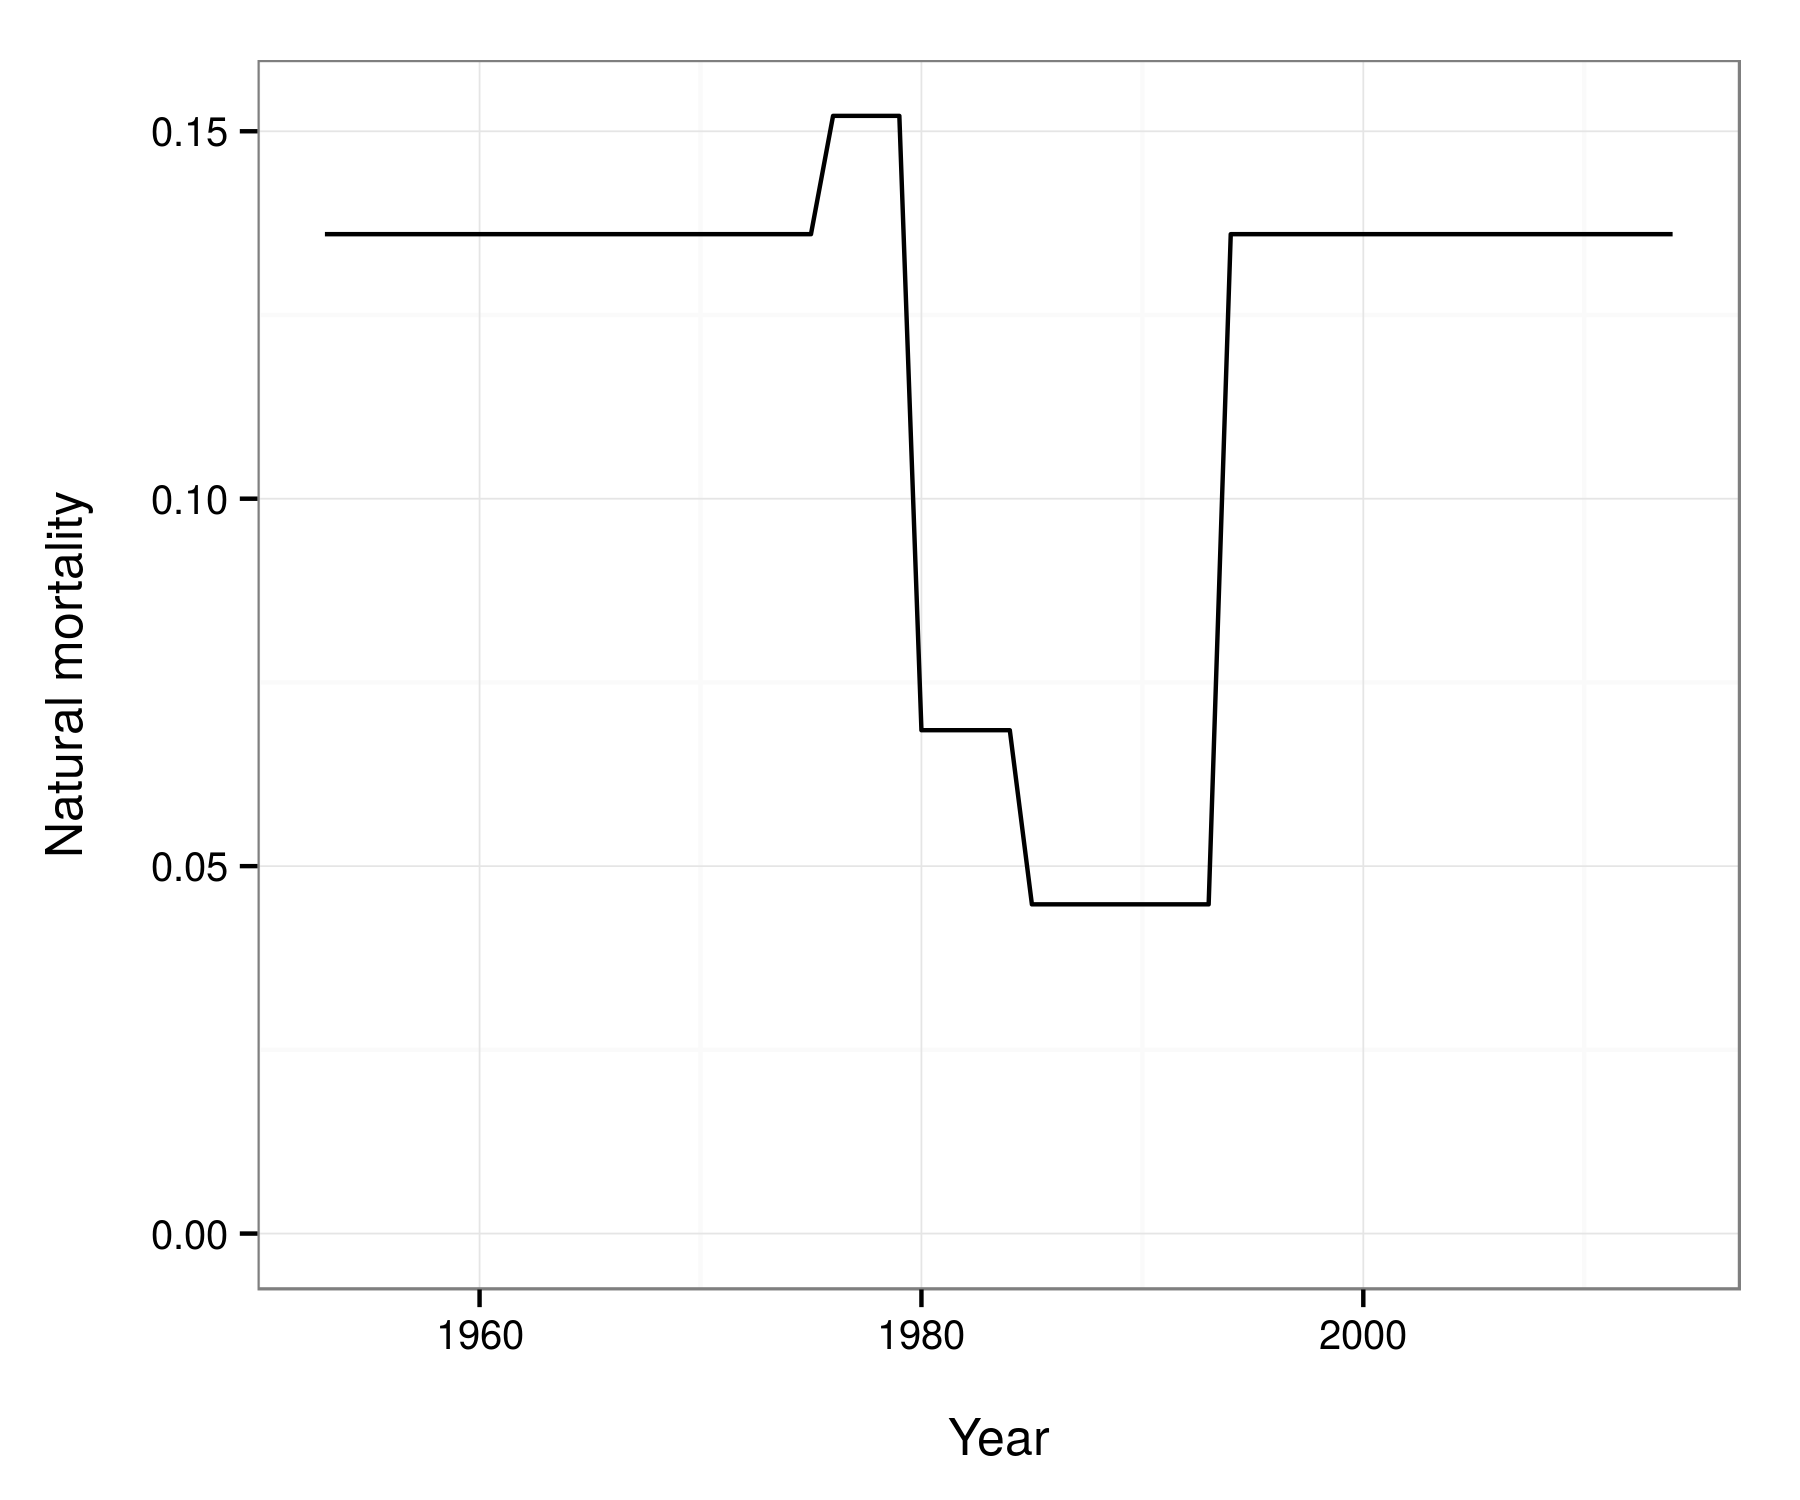
\includegraphics[width=0.65\linewidth]{figure/M_t_block.png}
\end{figure}
\end{frame}

%% =========================================================================== %%
%% =========================================================================== %%

\section{Selectivity, retention, fishing}

%% =========================================================================== %%
%% =========================================================================== %%

\subsection{Selectivity and retention}
\begin{frame}
\frametitle{Selectivity, retention and fishing mortality}
\begin{table}
  \centering
  \begin{tabular}{ccl}
  \hline
  Symbol & Dimensions & Description \\
  \hline
      \textcolor{red}{$a_{h,i,k}$} & $1$ & Length at 50\% selectivity \\
      \textcolor{red}{$\sigma^s_{h,i,k}$} & $1$ & Standard deviation in length at selectivity \\
      $\boldsymbol{s}_{h,i,k}$ & $\ell \times 1$ & Length at 50\% selectivity in length interval $\ell$ \\
      \textcolor{red}{$r_{h,i,k}$} & $1$ & Length at 50\% \\
      \textcolor{red}{$\sigma^y_{h,i,k}$} & $1$ & Standard deviation in length at retention \\
      $\boldsymbol{y}_{h,i,k}$ & $\ell \times 1$ & Length at 50\% retention in length interval $\ell$ \\
      \textcolor{blue}{$\xi_{i,k}$} & $1$ & Discard mortality rate for gear $k$
      in year $i$ \\
      $\boldsymbol\nu_{h,i,k}$ & $\ell \times 1$ & Vulnerability due to fishing mortality for sex $h$ \\
      \textcolor{red}{$\bar{\boldsymbol{f}}_k$} & $i \times 1$ & Average fishing mortality rate for gear $k$ \\
      \textcolor{red}{$\boldsymbol\Psi_{i,k}$} & & Fishing mortality deviate for gear $k$ in year $i$ \\
      \textcolor{red}{$\boldsymbol{F}_{i,k}$} & & Annual fishing mortality rate for gear $k$ in year $i$ \\
  \hline
  \end{tabular}
\end{table}
\end{frame}

%% =========================================================================== %%

\begin{frame}
\frametitle{Selectivity and retention}
The probability of catching an animal of sex $h$, in year $i$, in fishery $k$,
of length $\ell$ (i.e. selectivity) is
\begin{equation*}
  \boldsymbol{s}_{h,i,k} = \left(1 + \exp \left(-(\ell - \textcolor{red}{a_{h,i,k}}) /
  \textcolor{red}{\sigma_{h,i,k}^s} \right) \right)^{-1}.
\end{equation*}

The probability of an animal of sex $h$, in year $i$, in fishery $k$, of length
$\ell$ being retained is
\begin{equation*}
  \boldsymbol{y}_{h,i,k} = \left(1 + \exp \left(-(\textcolor{red}{r_{h,i,k}} - \ell \right) /
  \textcolor{red}{\sigma_{h,i,k}^y}) \right)^{-1}.
\end{equation*}
\end{frame}

%% =========================================================================== %%

\begin{frame}
\frametitle{Selectivity, retention and fishing mortality}
The joint probability of vulnerability due to fishing and discard mortality
is
\begin{equation*}
  \boldsymbol\nu_{h,i,k} = \boldsymbol{s}_{h,i,k} \left[ \boldsymbol{y}_{h,i,k} + (1 - \boldsymbol{y}_{h,i,k})
    \textcolor{blue}{\xi_{i,k}} \right],
\end{equation*}
where $\textcolor{blue}{\xi_{i,k}}$ is the discard mortality rate for fishery $k$ in
year $i$. Finally the fishing mortality is calculated as
\begin{align*}
  \textcolor{red}{\boldsymbol{F}_{h,i}} &= \sum_k \exp \left(
    \textcolor{red}{\bar{\boldsymbol{f}}_k} +
    \textcolor{red}{\boldsymbol\Psi_{i,k}} \right) \boldsymbol\nu_{h,i,k},\\
\end{align*}
The vector $\textcolor{red}{\boldsymbol{F}_{h,i}}$ represents all mortality
associated with fishing, including discards in directed and non-directed
fisheries.
\end{frame}

%% =========================================================================== %%

\begin{frame}
\frametitle{Selectivity and retention}
Assuming that selectivity for the NMFS trawl fishery is split into two blocks
(1975-1981 and 1982-2014) and that retention is constant with time
$\boldsymbol{y}_{h,i,k} = \boldsymbol{y}_{h,k}$
\begin{figure}[!htbp]
  \centering
  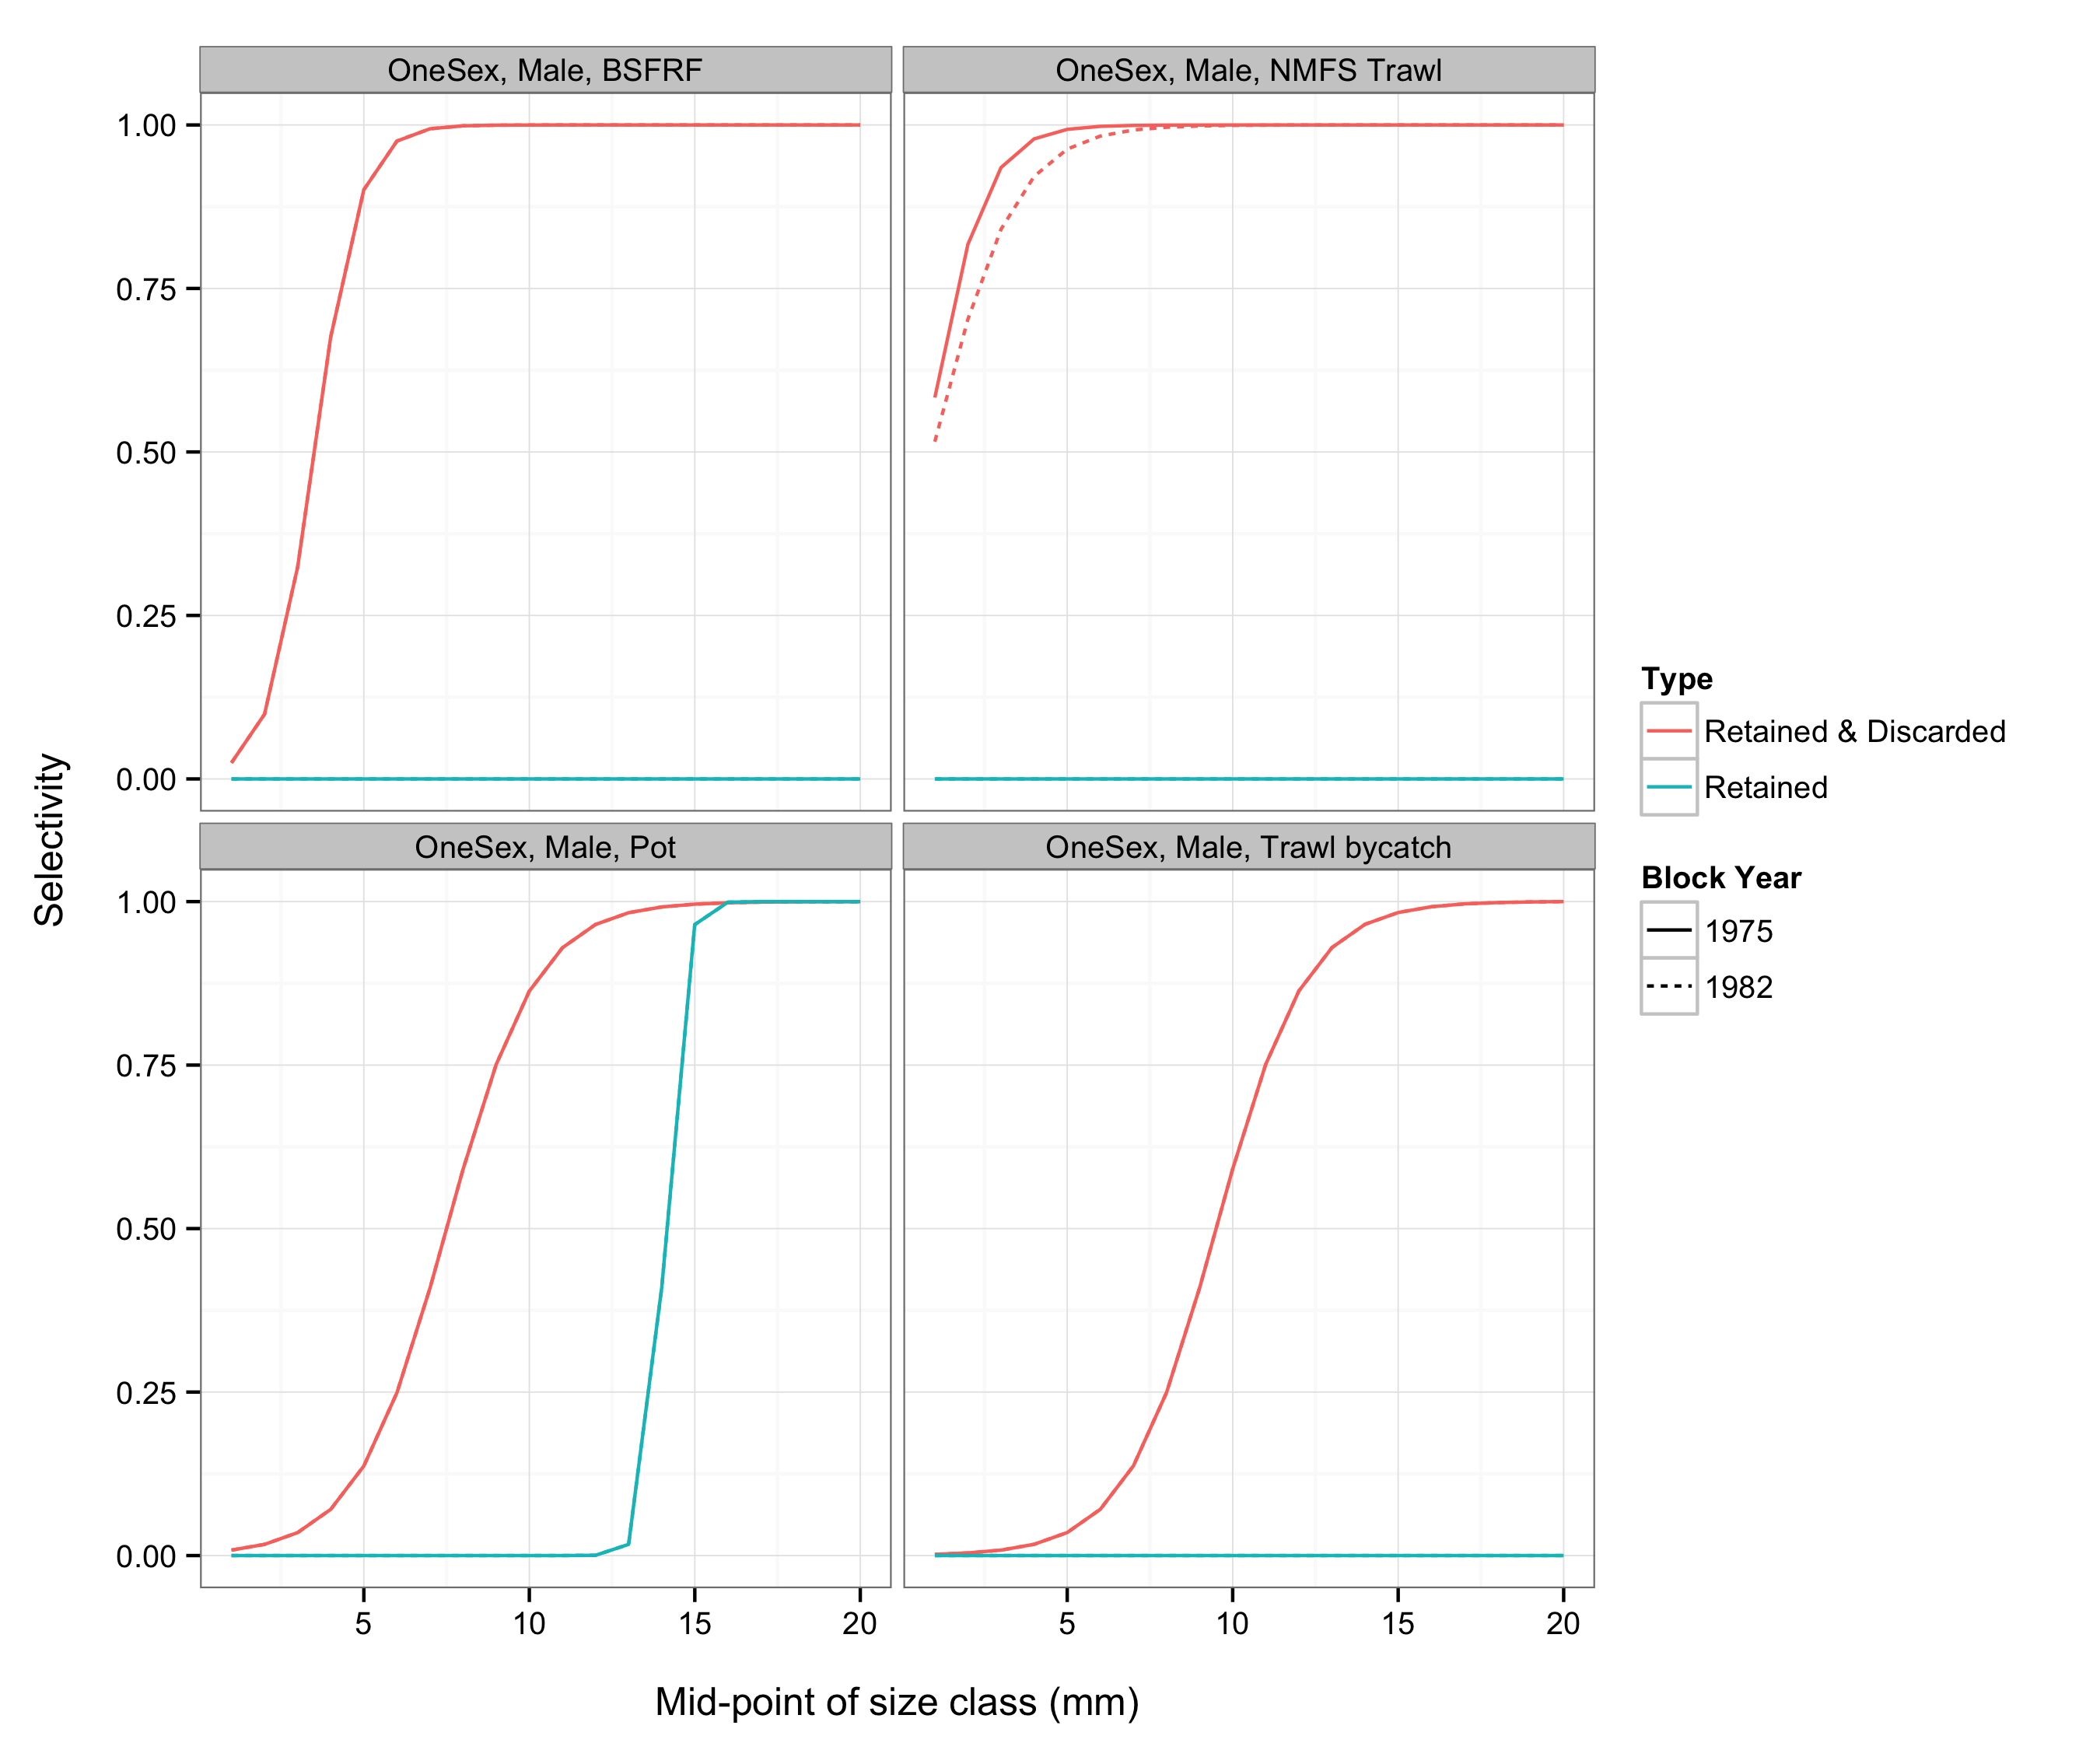
\includegraphics[width=0.6\linewidth]{../../examples/bbrkc/OneSex/figure/selectivity.png}
\end{figure}
\end{frame}

%% =========================================================================== %%
%% =========================================================================== %%

\section{Recruitment}

%% =========================================================================== %%
%% =========================================================================== %%

\begin{frame}
\frametitle{Recruitment}
Recruitment size-distribution
\begin{align*}
  \textcolor{red}{\alpha} &= \frac{\textcolor{red}{\alpha_r}}{\textcolor{red}{\beta_r}},\\
  p[x_\ell-0.5 \Delta x \le x \le x_\ell+0.5 \Delta x] &= p[x] = \int^{x_\ell+0.5
    \Delta x}_{x_\ell-0.5 \Delta x} \frac{ x^{\textcolor{red}{\alpha} - 1} \exp
    \left( \frac{x}{\textcolor{red}{\beta_r}} \right)}
    {\Gamma (\textcolor{red}{\alpha}) x^{\textcolor{red}{\alpha}}} dx.
\end{align*}
Initial recruitment
\begin{equation*}
  \boldsymbol{r}_{h,i} = 0.5 p[x] \textcolor{red}{\ddot{R}} \quad \text{for} \quad i=1.
\end{equation*}
Recruitment
\begin{equation*}
  \boldsymbol{r}_{h,i} = 0.5 p[x] \textcolor{red}{\bar{R}} e^{\delta_i}  \quad \text{for} \quad i>1,
\end{equation*}
where
\begin{equation*}
  \delta_i = \log (r_i) - (1-\rho) \log (\textcolor{red}{\bar{R}}) - \rho \log(r_{i-1}) + 0.5 \sigma^2_R
\end{equation*}
and
\begin{equation*}
  r_i = \sum_h r_{h,i}.
\end{equation*}
\end{frame}

%% =========================================================================== %%

\begin{frame}
\frametitle{Recruitment}
\begin{figure}[!htbp]
  \centering
  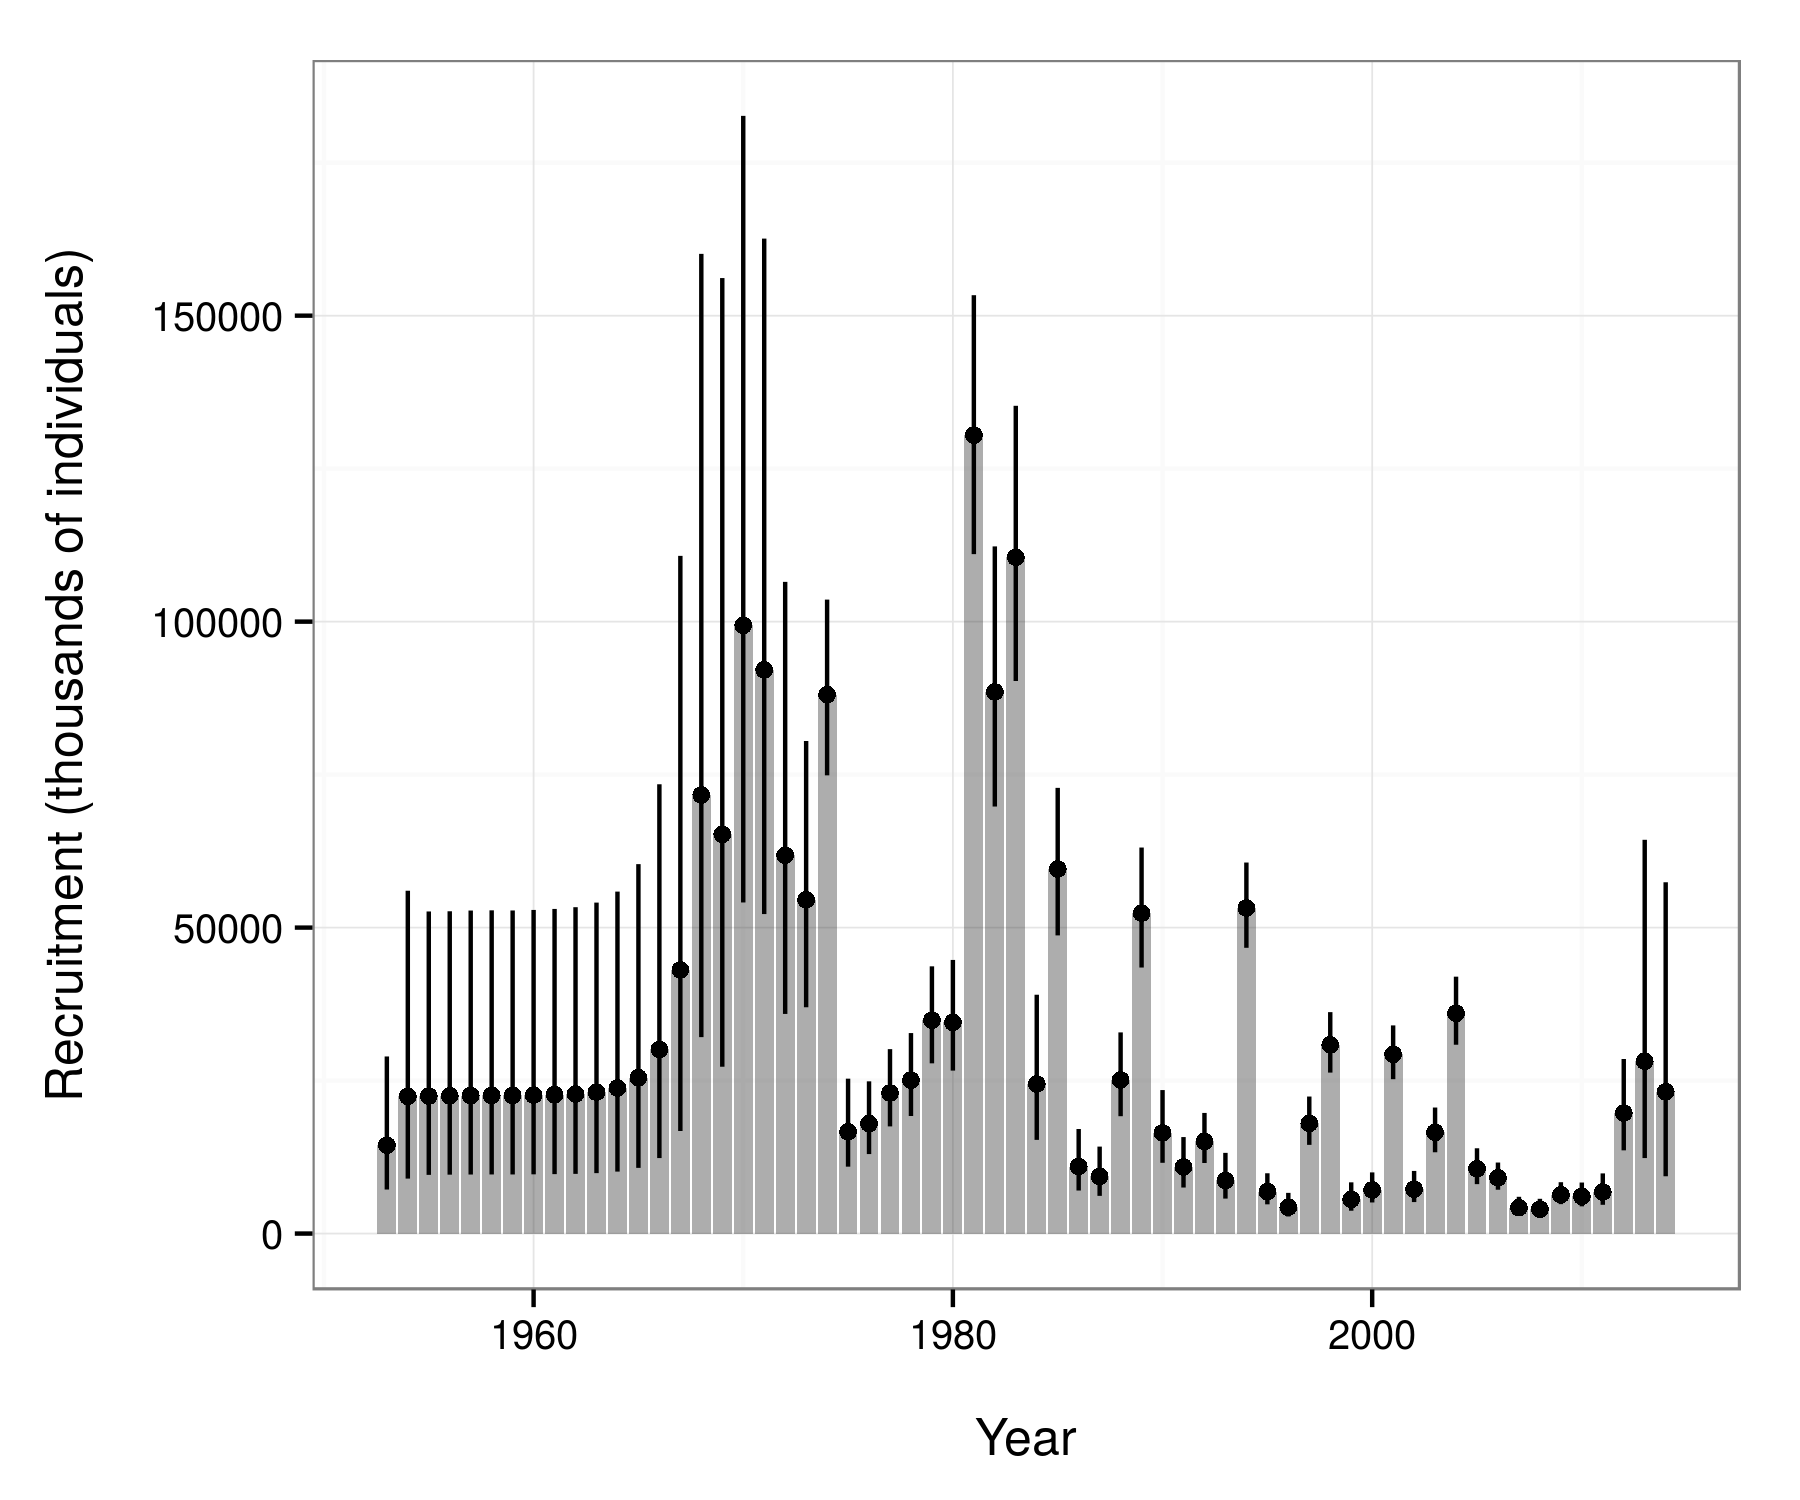
\includegraphics[width=0.75\linewidth]{../../examples/bbrkc/OneSex/figure/recruitment.png}
\end{figure}
\end{frame}

%% =========================================================================== %%
%% =========================================================================== %%

\section{Population dynamics}

%% =========================================================================== %%
%% =========================================================================== %%

\begin{frame}
\frametitle{Population dynamics}
Growth and survival process are combined, represented by
\begin{equation*}
  \boldsymbol{A}_{h,i} =
  \begin{cases}
    \boldsymbol{G}_{h} \left[ \exp(- \textcolor{red}{M_{h,i}}) \boldsymbol{I} \right] \quad  \text{for} \quad i = 1\\
    \boldsymbol{G}_{h} \left[ \exp(-\textcolor{red}{\boldsymbol{Z}_{h,i}}) \boldsymbol{I} \right] \quad \text{for} \quad i > 1
  \end{cases}.
\end{equation*}
where
\begin{equation*}
  \textcolor{red}{\boldsymbol{Z}_{h,i}} = \textcolor{red}{M_{h,i}} +
  \textcolor{red}{\boldsymbol{F}_{h,i}}.
\end{equation*}

Assuming unit recruitment, then the growth and survivorship in unfished and
fished conditions is given by the solutions to the equations
\begin{equation*}
  \boldsymbol{u}_{h,i} = -(\boldsymbol{A}_{h,i} - \boldsymbol{I})^{-1} (p[x])
  \quad \forall i.
\end{equation*}
The vector $\boldsymbol{u}_{h,i}$ represent the unique equilibrium solution for the
numbers per recruit in each size category.
\end{frame}

%% =========================================================================== %%

\begin{frame}
\frametitle{Initial population}
The mean weight at length ($\ell$) by sex ($h$) is represented by the $\ell
\times 1$ vector $\boldsymbol{w}_{h}$ and can take any form the user wishes
\begin{equation*}
  \boldsymbol{w}_{h} = f_w(\ell,\theta)
\end{equation*}

Similarly, the average proportion mature at length ($\ell$) by sex ($h$) is
represented by the $\ell \times 1$ vector $\boldsymbol{w}_{h}$ and can take any
form the user wishes
\begin{equation*}
  \boldsymbol{m}_{h} = f_m(\ell,\theta)
\end{equation*}

Steady-state conditions
\begin{equation*}
  B_0 = \textcolor{red}{R_0} \sum_h \lambda_h \sum_\ell \boldsymbol{u}_{h,i}
  \boldsymbol{w}_{h} \boldsymbol{m}_{h} \quad \text{for} \quad i=1,
\end{equation*}
\begin{equation*}
  \tilde{B} = \tilde{R} \sum_h \lambda_h \sum_\ell \boldsymbol{u}_{h,i} \boldsymbol{w}_{h}
  \boldsymbol{m}_{h} \quad \text{for} \quad i>1.
\end{equation*}
\end{frame}

%% =========================================================================== %%

\begin{frame}
\frametitle{Population evolution}
The total unfished numbers in each size category is defined as $R_0
\boldsymbol{u}_{h,i=1}$. Initial numbers at length
\begin{equation*}
  \boldsymbol{n}_{h,i} = \left[-\left( \boldsymbol{A}_{h} - \boldsymbol{I}
    \right)^{-1} \boldsymbol{r}_{h,i} \right] e^{\textcolor{red}{\boldsymbol\varepsilon}} \quad
  \text{for} \quad i=1,
\end{equation*}
where $\textcolor{red}{\boldsymbol\varepsilon}$ is an $\ell \times 1$ vector of
initial recruitment deviates. The numbers in each size-class in the following
time-step ($\boldsymbol{n}_{h,i+1}$) is the product of the numbers in each
size-class in the previous time-step ($\boldsymbol{n}_{h,i}$), size-specific
growth and survival ($\boldsymbol{A}_{h,i}$), plus new recruits
($\boldsymbol{r}_{h,i}$)
\begin{equation*}
  \boldsymbol{n}_{h,i+1} = \boldsymbol{n}_{h,i} \boldsymbol{A}_{h,i} +
  \boldsymbol{r}_{h,i} \quad \text{where} \quad i \ge 1.
\end{equation*}
\end{frame}

%% =========================================================================== %%
%% =========================================================================== %%

\section{Likelihoods}

%% =========================================================================== %%
%% =========================================================================== %%

\begin{frame}
\frametitle{Likelihoods and penalties}
Likelihoods
\begin{itemize}
\item likelihood of catch
\item likelihood of relative abundance
\item likelihood of size compositions
\item likelihood of recruitment deviations
\item likelihood of growth increment data
\end{itemize}
Penalties
\begin{itemize}
\item constrain $\log (\textcolor{red}{\Psi_{i,k}})$ to ensure they sum to zero
\item constrain mean \textcolor{red}{$\bar{\boldsymbol{f}}_k$} to regularize the
  solution
\item constrain $\textcolor{red}{M_{h,i}}$ in random walk
\end{itemize}

\end{frame}

%% =========================================================================== %%

\begin{frame}
\frametitle{Log-likelihood: catch}
The standard deviation of the catch ($\textcolor{blue}{\sigma_{i,k}}$) is calculated
from the CV as
\begin{equation*}
  \textcolor{blue}{\sigma_{i,k}} = \sqrt{\log \left( 1+\textcolor{blue}{c_{i,k}}^2 \right)}.
\end{equation*}
The expected catch is calculated using the Baranov catch equation
\begin{equation*}
  \hat{C}_{i,k} = \sum_{\ell} \left[ \boldsymbol{n}_{h,i} \boldsymbol{w}_{h}
    \frac{\textcolor{red}{\boldsymbol{F}_{h,i}}}{\textcolor{red}{\boldsymbol{Z}_{h,i}}} 
    \left( 1 - e^{-\textcolor{red}{\boldsymbol{Z}_{h,i}}} \right) \right] \quad \text{where}
  \quad \textcolor{red}{\boldsymbol{Z}_{h,i}}
  = \textcolor{red}{M_{h,i}} + \textcolor{red}{\boldsymbol{F}_{h,i}}.
\end{equation*}
The log-likelihood is
\begin{equation*}
  \ell(\textcolor{green}{C_{i,k}}) = 0.5 \log (2 \pi) + \log
  (\textcolor{blue}{\sigma_{i,k}}) -
  \frac{1}{2\textcolor{blue}{\sigma_{i,k}}^2} (\textcolor{green}{C_{i,k}} - \hat{C}_{i,k})^2.
\end{equation*}
\end{frame}

%% =========================================================================== %%

\begin{frame}
\frametitle{Log-likelihood: catch}
\begin{figure}[!htbp]
  \centering
  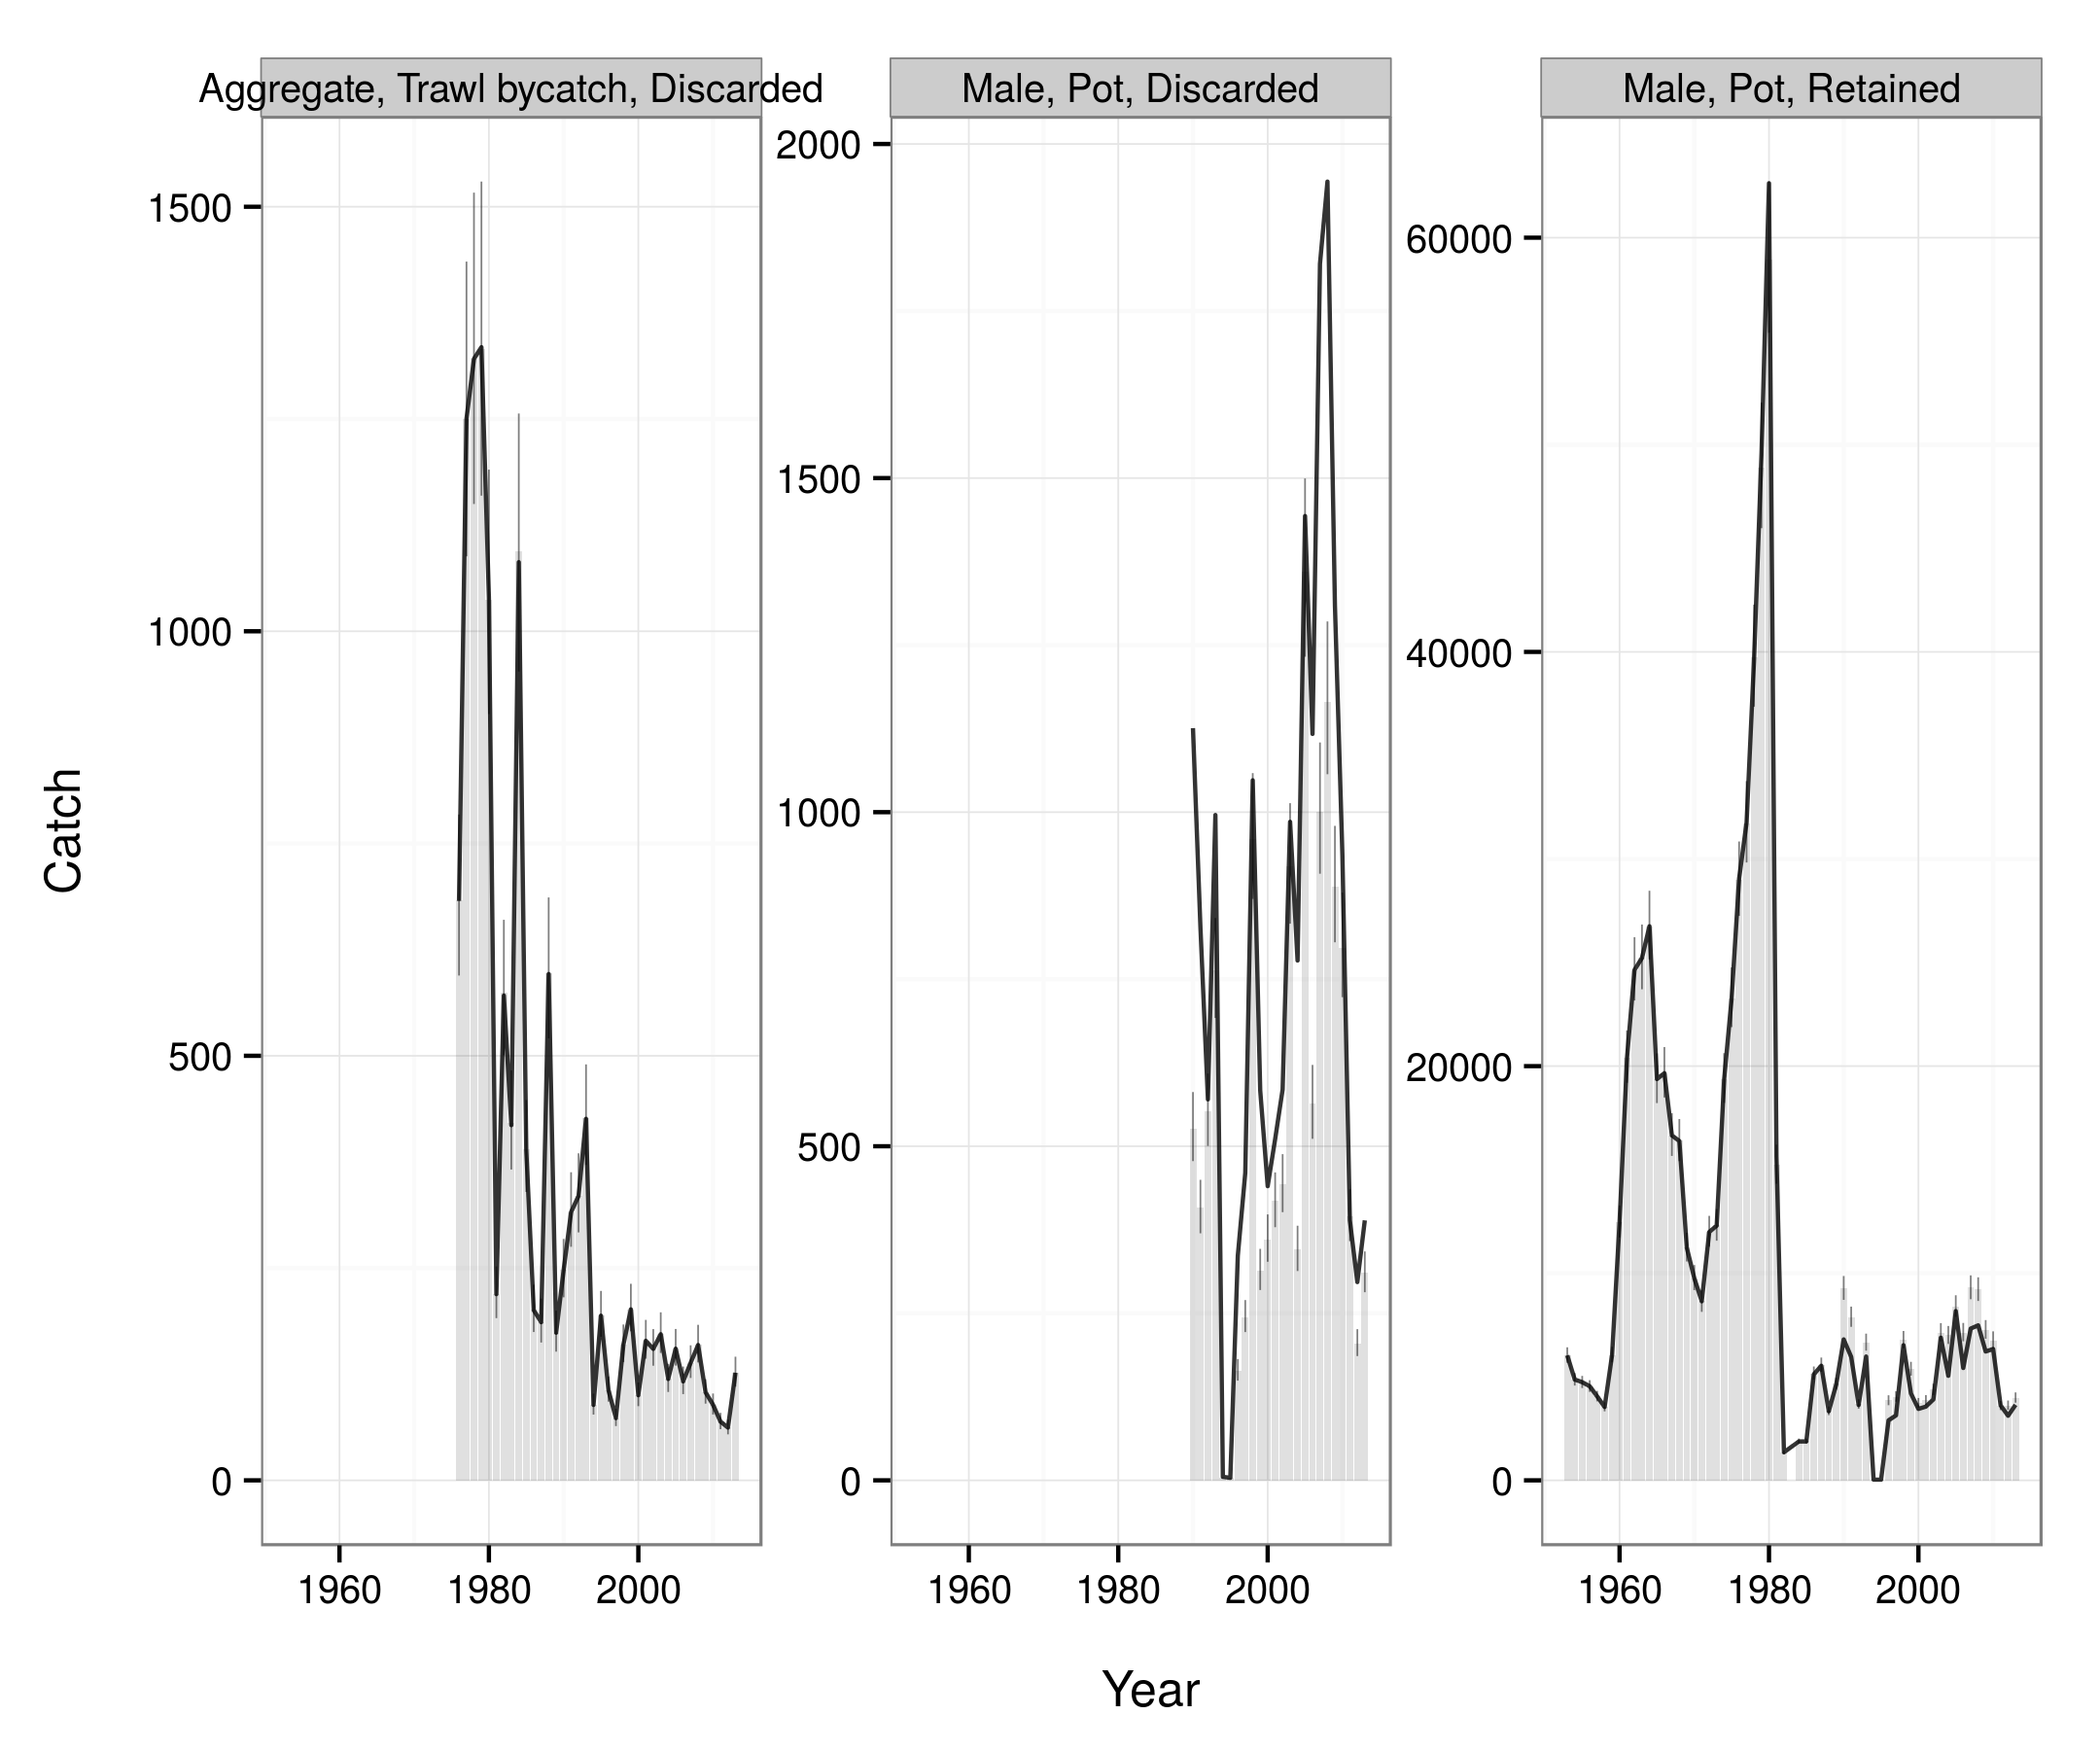
\includegraphics[width=0.75\linewidth]{../../examples/bbrkc/OneSex/figure/catch.png}
\end{figure}
\end{frame}

%% =========================================================================== %%

\begin{frame}
\frametitle{Log-likelihoods: relative abundance}
The catchability coefficient $q$ is treated as a nuisance parameter and
integrated out of the model~\citep{Walters1994}.
\begin{equation*}
  q = \exp \left( \frac{1}{n} \sum_i \log \left(
      \frac{\textcolor{green}{I_i}}{V_i} \right) \right).
\end{equation*}
The standard deviation ($\textcolor{blue}{\sigma_{i,k}}$) is calculated from the CV as
\begin{equation*}
  \textcolor{blue}{\sigma_{i,k}} = \sqrt{\log \left(
      1+\textcolor{blue}{c_{i,k}}^2 \right)}.
\end{equation*}
The log-likelihood is
\begin{equation*}
  \ell(\textcolor{green}{I_{i,k}}) = \lambda \left( 0.5 \log (2 \pi) + \log
  (\textcolor{blue}{\sigma_{i,k}}) +
  \frac{1}{2\textcolor{blue}{\sigma^2_{i,k}}} (\textcolor{green}{I_{i,k}} -
  qV_{i,k})^2 \right).
\end{equation*}
\end{frame}

%% =========================================================================== %%

\begin{frame}
\frametitle{Log-likelihood: relative abundance}
\begin{figure}[!htbp]
  \centering
  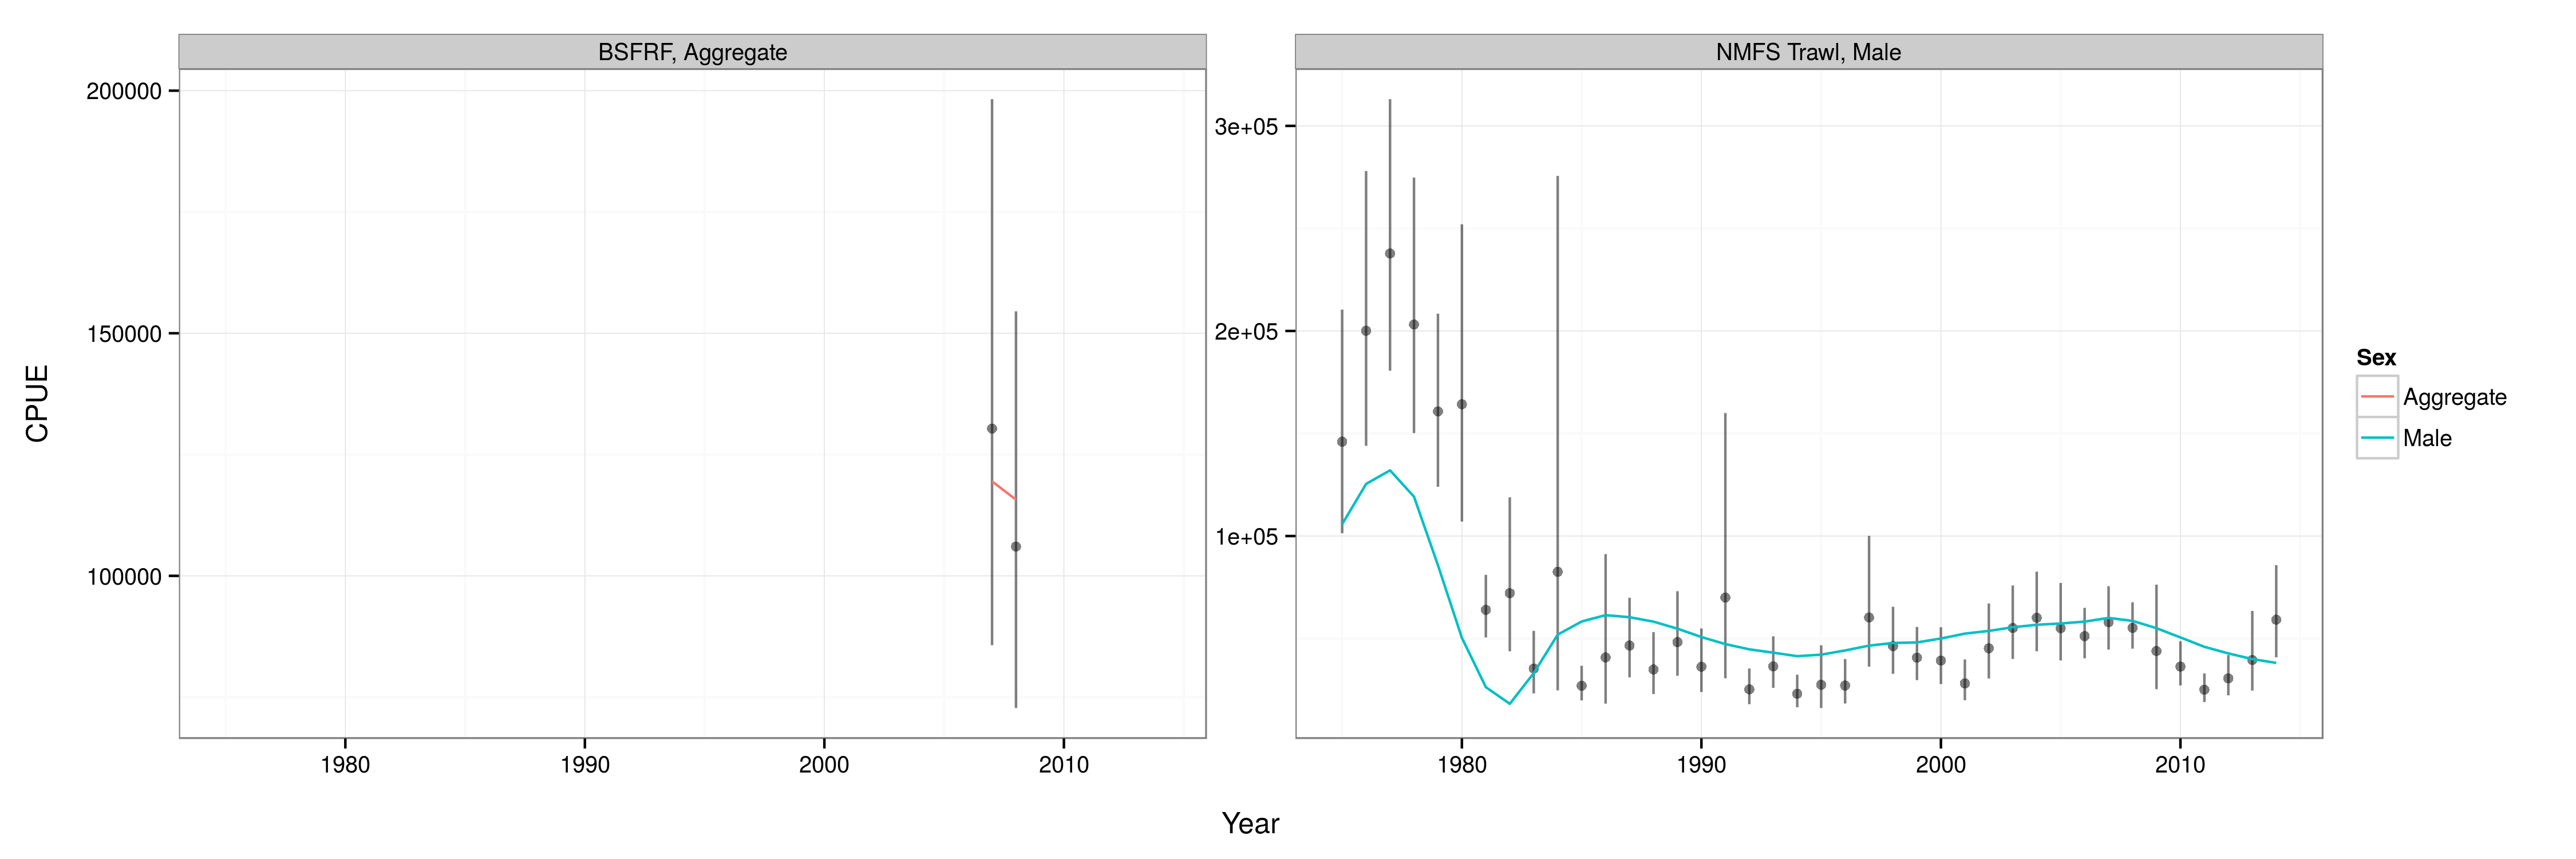
\includegraphics[width=\linewidth]{../../examples/bbrkc/OneSex/figure/cpue.png}
\end{figure}
\end{frame}

%% =========================================================================== %%

\begin{frame}
\frametitle{Log-likelihoods: size composition}
Size composition data is assumed to be multinomial distributed
\begin{equation*}
  \boldsymbol{P}_{h,i} = (P_\ell)_{h,i} = \mathcal{M}\text{ultinomial} \left( n_{h,i},
  \boldsymbol{Q}_{h,i} \right)
\end{equation*}

Alternatively we could use
\begin{equation*}
  \boldsymbol{P}_{h,i} = (P_\ell)_{h,i} = \mathcal{D}\text{irichlet} \left(
    \textcolor{red}{\lambda_0} \textcolor{blue}{n_{h,i}} \boldsymbol{Q}_{h,i} \right).
\end{equation*}
In this context, $\textcolor{red}{\lambda_0}$ can be thought of as the data
weight (which may be estimated in the model) and $n_{h,i}$ is the relative
sample size between years.
\end{frame}

%% =========================================================================== %%

\begin{frame}
\frametitle{Log-likelihoods}
Natural mortality
\begin{equation*}
  \ell(\textcolor{red}{M_{h,i}}) = 
  0.5 \log (2 \pi) + \log (\textcolor{blue}{\sigma_{M}}) + 0.5
  \frac{1}{\textcolor{blue}{\sigma^2_{M}}} \sum_i
  \delta_i^2.
\end{equation*}
\end{frame}

%% =========================================================================== %%

\begin{frame}
\frametitle{References}
\bibliographystyle{agsm}
\bibliography{../references/Gmacs}
\end{frame}

%% =========================================================================== %%

\end{document}




%% =========================================================================== %%

\subsection{Log-likelihoods}
\begin{frame}
\frametitle{Log-likelihood: normal}
In general, if we have a random variable $x$ that is normally distributed with
mean $\mu$ and variance $\sigma^2$, we write
\begin{equation*}
  x \sim \mathcal{N} \left(\mu, \sigma^2 \right).
\end{equation*}
The log-likelihood is
\begin{equation*}
  \ell(\mu,\sigma^2; x_1,\ldots,x_n) = \cancel{-\frac{n}{2} \log (2 \pi)} - n \log (\sigma) -
  \frac{1}{2\sigma^2} \sum_i^n (x_i - \mu)^2.
\end{equation*}
If a coefficient of variation $c$ is defined, rather than a standard deviation
$\sigma$ we write
\begin{equation*}
  \sigma = \sqrt{\log \left( 1+c^2 \right)}.
\end{equation*}
\end{frame}

%% =========================================================================== %%

\begin{frame}
\frametitle{Log-likelihood: lognormal}
In general, if we have a random variable $x$ that is log-normally distributed
with location $\mu$ and scale $\sigma$, we write
\begin{equation*}
  x \sim \log \mathcal{N} \left(\mu, \sigma^2 \right).
\end{equation*}
The log-likelihood is
\begin{equation*}
  \ell(\mu,\sigma^2; x_1,\ldots,x_n) = 0.5 \log (2 \pi) + \log (\sigma) + \log
  (x) + \frac{1}{2\sigma^2} (x - \mu)^2.
\end{equation*}
\end{frame}
